% LaTeX source for ``Think Stats:
% Probability and Statistics for Programmers''
% Copyright 2010  Allen B. Downey.

% License: Creative Commons Attribution-Share Alike 3.0 Unported
% http://creativecommons.org/licenses/by-sa/3.0/
%

%\documentclass[10pt,b5paper]{book}
\documentclass[10pt]{book}
\usepackage[width=5.5in,height=8.5in,
  hmarginratio=3:2,vmarginratio=1:1]{geometry}

% for some of these packages, you might have to install
% texlive-latex-extra (in Ubuntu)

\usepackage{pslatex}
\usepackage{url}
\usepackage{fancyhdr}
\usepackage{graphicx}
\usepackage{amsmath, amsthm, amssymb}
\usepackage{exercise}                        % texlive-latex-extra
\usepackage{makeidx}
\usepackage{setspace}
\usepackage{hevea}                           
\usepackage{upquote}

\title{Think Stats}
\newcommand{\thetitle}{Think Stats: Probability and Statistics for Programmers}
\newcommand{\theversion}{1.0.1}

% these styles get translated in CSS for the HTML version
\newstyle{a:link}{color:black;}
\newstyle{p+p}{margin-top:1em;margin-bottom:1em}
\newstyle{img}{border:0px}

% change the arrows in the HTML version
\setlinkstext
  {\imgsrc[ALT="Previous"]{back.png}}
  {\imgsrc[ALT="Up"]{up.png}}
  {\imgsrc[ALT="Next"]{next.png}} 

\makeindex

\begin{document}

\frontmatter

% LATEXONLY

\input{latexonly}

\newtheorem{ex}{Exercise}[chapter]

\begin{latexonly}

\renewcommand{\blankpage}{\thispagestyle{empty} \quad \newpage}

%\blankpage
%\blankpage

% TITLE PAGES FOR LATEX VERSION

%-half title--------------------------------------------------
\thispagestyle{empty}

\begin{flushright}
\vspace*{2.0in}

\begin{spacing}{3}
{\huge Think Stats: Probability and Statistics for Programmers}\\
{\Large }
\end{spacing}

\vspace{0.25in}

Version \theversion

\vfill

\end{flushright}

%--verso------------------------------------------------------

\blankpage
\blankpage
%\clearemptydoublepage
%\pagebreak
%\thispagestyle{empty}
%\vspace*{6in}

%--title page--------------------------------------------------
\pagebreak
\thispagestyle{empty}

\begin{flushright}
\vspace*{2.0in}

\begin{spacing}{3}
{\huge Think Stats}\\
{\Large Probability and Statistics for Programmers}
\end{spacing}

\vspace{0.25in}

Version \theversion

\vspace{1in}


{\Large
Allen Downey\\
}


\vspace{0.5in}

{\Large Green Tea Press}

{\small Needham, Massachusetts}

%\includegraphics[width=1in]{figs/logo1.eps}
\vfill

\end{flushright}


%--copyright--------------------------------------------------
\pagebreak
\thispagestyle{empty}

{\small
Copyright \copyright ~2010 Allen Downey.


\vspace{0.2in}

\begin{flushleft}
Green Tea Press       \\
9 Washburn Ave \\
Needham MA 02492
\end{flushleft}

Permission is granted to copy, distribute, and/or modify this document
under the terms of the Creative Commons Attribution-Share Alike 3.0 Unported
License, which is available at \url{creativecommons.org/licenses/by-sa/3.0/}.

The original form of this book is \LaTeX\ source code.  Compiling this
code has the effect of generating a device-independent representation
of a textbook, which can be converted to other formats and printed.

The \LaTeX\ source for this book is available from
\url{www.thinkstatsbook.com}.

The cover for this book is based on a photo by Paul Friel
(\url{flickr.com/people/frielp/}), who made it available under
the Creative Commons Attribution license.  The original photo
is at \url{flickr.com/photos/frielp/11999738/}.

\vspace{0.2in}

} % end small

\end{latexonly}


% HTMLONLY

\begin{htmlonly}

% TITLE PAGE FOR HTML VERSION

{\Large \thetitle}

{\large Allen B. Downey}

Version \theversion

\setcounter{chapter}{-1}

\end{htmlonly}


\chapter{Preface}
\label{preface}

\section*{Programming is a pedagogic wedge}

Operational thinking vs relational thinking

example: counting frequencies

Notation: math notation and programming languages are formal languages
designed for different purposes.

Often consistent, so translation can be straightforward.

Other examples are surprisingly different.

Math notation is concise and general-purpose but suffers from
ambiguity, sloppy typing, implied scoping, overloading, poor
readability

barrier for some people (more so than programming languages?)

Programs are executable, and therefore testable, which gives students
immediate feedback on their understanding of concepts.

Also lend themselves to empirical tests.

Probability is often tricky; hard to ``prove'' a result because it
is easy to write a bad proof.

A simulation can be a more compelling proof -- easier to read and check
correctness.  Erdos and the Monty Hall problem.

Comment on my vocabulary and notation: generally consistent with the
Wikipedia.


Allen B. Downey \\
Needham MA\\

Allen Downey is an Associate Professor of Computer Science at 
the Franklin W. Olin College of Engineering.




%\section*{Acknowledgements}



\section*{Contributor List}

\index{contributors}

If you have a suggestion or correction, please send email to 
{\tt downey@allendowney.com}.  If I make a change based on your
feedback, I will add you to the contributor list
(unless you ask to be omitted).

If you include at least part of the sentence the
error appears in, that makes it easy for me to search.  Page and
section numbers are fine, too, but not quite as easy to work with.
Thanks!

\small

\begin{itemize}

\item 

% ENDCONTRIB

\end{itemize}

\normalsize

\clearemptydoublepage

% TABLE OF CONTENTS
\begin{latexonly}

\tableofcontents

\clearemptydoublepage

\end{latexonly}

% START THE BOOK
\mainmatter


\chapter{Statistical thinking for programmers}
\label{intro}

This book is about turning data into knowledge.  Data is cheap (at
least relatively); knowledge is harder to come by.

I will present three related pieces:

\begin{description}

\item[Probability] is the study of random events.  Most people have an
  intuitive understanding of degrees of probability, which is why you
  can use words like ``probably'' and ``unlikely'' without special
  training, but we will talk about how to make quantitative claims
  about those degrees.

\item[Statistics] is the discipline of using data samples to support
  claims about populations.  Most statistical analysis is based on
  probability, which is why these pieces are usually presented
  together.

\item[Computation] is a tool that is well-suited to quantitative
  analysis, and computers are commonly used to process statistics.
  Also (and more importantly for this book) computational experiments
  are useful for exploring concepts in probability and statistics.

\end{description}

The thesis of this book is that if you know how to program, you can
use that skill to help you understand probability and statistics.
These topics are often presented from a mathematical perspective, and
that approach works well for some people.  But some important ideas
in this area are hard to work with mathematically and relatively
easy to approach computationally.

The rest of this chapter presents a case study motivated by a question
I heard when my wife and I were expecting our first child: do first
babies tend to arrive late?

\section{Do first babies arrive late?}

If you Google this question, you will find plenty of discussion.
Some people claim it's true, others say it's a myth, and some people
say it's the other way around: first babies come early.

In many of these discussions, people provide data to support their
claims.  I found many examples like these:

\begin{quote}

``My two friends that have given birth recently to their first babies,
BOTH went almost 2 weeks overdue before going into labour or being
induced.''

``My first one came 2 weeks late and now I think the second one is
going to come out two weeks early!!''

``I don't think that can be true because my sister was my mother's
first and she was early, as with many of my cousins.''

\end{quote}

Reports like these are called {\bf anecdotal evidence} because they
are based on data that is unpublished and usually personal.  In casual
conversation, there is nothing wrong with anecdotes, so I don't mean
to pick on the people I quoted.

But we might want evidence that is more persuasive and
an answer that is more reliable.  By those standards, anecdotal
evidence usually fails, because:

\begin{description}

\item[Small number of observations:] If the gestation period is longer
  for first babies, the difference is probably small compared to the
  natural variation.  In that case, we might have to compare a large
  number of pregnancies to be sure there is really a difference (or
  not).

\item[Selection bias:] People who join a discussion of this question
  might be interested because their first babies were late.  In that
  case the process of selecting data would bias the results.

\item[Confirmation bias:] People who believe the claim might be more
  likely to contribute examples that confirm it.  People who doubt the
  claim are more likely to cite counterexamples.

\item[Inaccuracy:] Anecotes are often personal stories that are
  (deliberately or not) misremembered, misrepresented, repeated
  inaccurately, etc.

\end{description}

So how can we do better?

\section{A statistical approach}

To address the limitations of anecdotes, we will use the tools
of statistics, which include:

\begin{description}

\item[Data collection:] We will use data from a large national survey
  that was designed explicitly with the goal of generating
  statistically valid inferences about the U.S. population.

\item[Descriptive statistics:] We will generate statistics that
  summarize the data concisely, and evaluate different ways to
  visualize data.

\item[Exploratory data analysis:] We will look for
  patterns, differences, and other features that address the questions
  we are interested in.  At the same time we will check for
  inconsistencies and identify limitations.

\item[Hypothesis testing:] Where we see apparent effects (like a
  difference between two groups), we will evaluate whether the effect
  is likely to be real, or whether it might have happened by chance.

\item[Estimation:] We will use data from a sample to estimate
  characteristics of the general population.

\end{description}

By performing these steps with care to avoid common pitfalls, we can
reach conclusions that are more justifiable and more likely to be
correct.


\section{The National Survey of Family Growth}

Since 1973 the U.S. Centers for Disease Control and Prevention (CDC)
have conducted the National Survey of Family Growth (NSFG),
which is intended to gather ``information on family life, marriage and
divorce, pregnancy, infertility, use of contraception, and men's and
women's health. The survey results are used ... to plan health services and
health education programs, and to do statistical studies of families,
fertility, and health.''\footnote{See
  \url{cdc.gov/nchs/nsfg.htm}.}

We will use data collected by this survey to investigate whether first
babies tend to come late, and other questions.  In order to use this
data effectively, we have to understand the design of the study.

The NSFG is a {\bf cross-sectional} study, which means that it
captures a snapshot of a group at a point in time.  The most
common alternative is a {\bf longitudinal} study, which observes a
group repeatedly over a period of time.

The NSFG has been conducted seven times; each deployment is called
a {\bf cycle}.  We will be using data from Cycle 6, which was
conducted from January 2002 to March 2003.

The goal of the survey is to draw conclusions about a
{\bf population}; the target population of the NSFG is people in
the United States aged 15-44.

The people who participate in a survey are called {\bf respondents}.
In general, cross-sectional studies are meant to be {\bf
  representative}, which means that every member of the target
population has an equal chance of participating.  Of course that ideal
is hard to achieve in practice, but people who conduct surveys come as
close as they can.

The NSFG not representative; instead it is deliberately {\bf
  oversampled}.  The designers of the study recruited three
groups---Hispanics, African-Americans and teenagers---at rates higher
than their representation in the U.S. population.
The reason for oversampling is to make sure that the number of
respondents in each of these groups is large enough to draw valid
statistical inferences.

Of course, the drawback of oversampling is that it is not as easy
to draw conclusions about the general population based on statistics
from the survey.  We will come back to this point later.

\begin{ex}

Although the NSFG has been conducted seven times, it is not a
longitudinal study.  Read the Wikipedia pages
\url{wikipedia.org/wiki/Cross-sectional_study}
and
\url{wikipedia.org/wiki/Longitudinal_study}
to make sure you understand why not.

\end{ex}

\begin{ex}

In this exercise, you will download data from the NSFG and do some
exploratory data analysis.

\begin{enumerate}

\item Go to \url{thinkstatsbook.com/nsfg.html}.  Read the terms of
use for this data and click ``I accept these terms'' (assuming that you do).

\item Download the files named {\tt 2002FemResp.dat.gz} and {\tt
  2002FemPreg.dat.gz}.  The first is the respondent file, which contains
  one line for each of the 7,643 female respondents.
  The second file contains one line for each pregnancy reported by a
  respondent.

\item Online documentation of the survey is at
  \url{nsfg.icpsr.umich.edu/cocoon/WebDocs/NSFG/public/index.htm}.
  Browse the sections in the left navigation bar to get a sense of
  what data are included.  You can also read the questionnaires
  at \url{cdc.gov/nchs/data/nsfg/nsfg_2002_questionnaires.htm}.

\item The web page for this book provides code to process the data
  files from the NSFG.  Download \url{thinkstatsbook.com/survey.py}
  and run it in the same directory you put the data files in.  It
  should read the data files and print the number of lines in each:

\begin{verbatim}
Number of respondents 7643
Number of pregnancies 13593
\end{verbatim}

\item Browse the code to get a sense of what it does.  The next
section explains how it works.

\end{enumerate}

\end{ex}

\section{Tables and records}

The poet-philosopher Steve Martin once said:

\begin{quote}
``Oeuf'' means egg, ``chapeau'' means hat.  It's like those French
  have a different word for everything.
\end{quote}

Like the French, database programmers speak a slightly
different language, and since we're working with a database we need
to learn some vocabulary.

Each line in the respondents file contains information about one
respondent.  This information is called a {\bf record}.  The
variables that make up a record are called {\bf fields}.  A
collection of records is called a {\bf table}.

If you read {\tt survey.py} you will see class definitions for {\tt
  Record}, which is an object that represents a record, and {\tt
  Table}, which represents a table.

There are two subclasses of
{\tt Record}, {\tt Respondent} and {\tt Pregnancy}, which
contain records from the respondent and pregnancy tables.
For the time being, these classes are empty; in particular, there
is no {\tt init} method to initialize their attributes.  Instead
we will use {\tt Table.MakeRecord} to convert a line of text into
a {\tt Record} object.

There are also two subclasses of {\tt Table}, {\tt Respondents}
and {\tt Pregnancies}.  The {\tt init} method in each class
specifies the default name of the data file and the type of
record to create.  Each {\tt Table} object has an attribute
named {\tt records}, which is a list of {\tt Record} objects.

For each {\tt Table}, the {\tt GetFields} method returns
a list of tuples that specify the fields from the record that
will be stored as attributes in each {\tt Record} object.  (You
might want to read that last sentence twice.)

For example, here is {\tt Pregnancies.GetFields}:

\begin{verbatim}
    def GetFields(self):
        return [
            ('caseid', 1, 12, int),
            ('prglength', 275, 276, int),
            ('outcome', 277, 277, int),
            ('birthord', 278, 279, int),
            ('finalwgt', 423, 440, float),
            ]
\end{verbatim}

The first tuple says that the field {\tt caseid} is in columns
1 through 12 and it's an integer.  Each tuple contains the following
information:

\begin{description}

\item[field:] The name of the attribute where the field
will be stored.  Most of the time I use the names from the
NSFG codebook, converted to all lower case.

\item[start:] The index of the starting column for this
field.  You can look up these indices in the NSFG codebook
at \url{nsfg.icpsr.umich.edu/cocoon/WebDocs/NSFG/public/index.htm}.
For example, the indices for {\tt caseid} are
1--12.

\item[end:] The index of the ending column for this
field.  Unlike in Python, the end index is inclusive.

\item[conversion function:] A function that takes a string
and converts it to an appropriate type.  You can use built-in
functions, like {\tt int} and {\tt float}, or user-defined
functions.  If the conversion fails, the attribute gets the
string value {\tt 'NA'}.  If you don't want to convert a
field, you can provide an identity function or use {\tt str}.

\end{description}

For pregnancy records, we extract the following variables:

\begin{description}

\item[caseid] is the integer ID of the respondent.

\item[prglength] is the integer duration of the pregnancy in weeks.

\item[outcome] is an integer code for the outcome of the pregnancy.
The code 1 indicates a live birth.

\item[birthord] is the integer birth order of each live birth;
for example, the code for a first child is 1. 
For outcomes other than live birth, this field is blank.

\item[finalwgt] is the statistical weight associated with the respondent.
It is a floating-point value that indicates the number of people in
the U.S. population this respondent represents.  Members of undersampled
groups have higher weights.

\end{description}

If you read the casebook carefully, you will see that most of these
variables are {\bf recodes}, which means that they are not part
of the {\bf raw data} collected by the survey, but they are
calculated using the raw data.

For example, {\tt prglength} for live births is equal to the raw
variable {\tt wksgest} (weeks of gestation) if it is available;
otherwise it is estimated using {\tt mosgest * 4.33} (months of
gestation times the average number of weeks in a month).

Recodes are often based on logic that checks the consistency and
accuracy of the data.  In general it is a good idea to use recodes
unless there is a compelling reason to process the raw data
yourself.

\begin{ex}

In this exercise you will write a program to explore the data
in the Pregnancies table.

\begin{enumerate}

\item In the directory where you put {\tt survey.py} and the
data files, create a file named \verb"first.py" and
type or paste in the following code:

\begin{verbatim}
import survey
table = survey.Pregnancies()
table.ReadRecords()
print 'Number of pregnancies', len(table.records)
\end{verbatim}

The result should be 13593 pregnancies.

\item Write a loop that iterates \verb"table" and counts
the number of live births.  Find the documentation of {\tt outcome}
and confirm that your result is consistent with the summary
in the documentation.

\item Modify the loop to partition the live birth records into
two groups, one for first babies and one for the others.  Again,
read the documentation of {\tt birthord} to see if your results
are consistent.

When you are working with a new dataset, these kinds of checks
are useful for finding errors and inconsistencies in the data,
detecting bugs in your program, and checking your understanding
of the way the data are encoded.

\item Compute the average pregnancy length (in weeks) for first
babies and others.  Is there a difference between the groups?  How
big is it?

Note: For now we are ignoring the {\tt finalwgt} variable.

\end{enumerate}

You can download a solution to this exercise from
\url{thinkstatsbook.com/first.py}.

\end{ex}

\section{Significance}

In the previous exercise, you compared the gestation period for first
babies and others; if things worked out, you found that first
babies are born about 13 hours later, on average.

A difference like that is called an {\bf apparent effect}; that is,
there might be something going on, but we are not yet sure.  There are
several questions we still want to ask:

\begin{itemize}

\item If the two groups have different means, what about other {\bf
  summary statistics}, like median and variance?  Can we be more
  precise about how the groups differ?

\item Is it possible that the difference we saw could occur by chance,
  even if the groups we compared were actually the same?  If so,
  we would conclude that the effect was not {\bf statistically
    significant}.

\item Is it possible that the apparent effect is due to sample bias or
  some other error in the experimental setup?  If so, then we might
  conclude that the effect is an {\bf artifact}; that is, something we
  created (by accident) rather than found. 

\end{itemize}

We will address these questions in the next few chapters.

\section{Glossary}

\begin{description}

\item[anecdotal evidence:] Evidence, often personal, that is collected
  casually rather than by a well-designed study.

\item[population:] A group we are interested in studying, often a
  group of people, but the term is also used for animals, vegetables
  and minerals\footnote{If you don't recognize this phrase, see
    \url{wikipedia.org/wiki/Twenty_Questions}.}.

\item[cross-sectional study:] A study that collects data about a
population at a particular point in time.

\item[longitudinal study:] A study that follows a population over
time, collecting data from the same group repeatedly.

\item[respondent:] A person who responds to a survey.

\item[sample:] The subset of a population used to collect data.

\item[representative:] A sample is representative if every member
of the population has the same chance of being in the sample.

\item[oversampling:] The technique of increasing the representation
of a sub-population in order to avoid errors due to small sample
sizes.

\item[record:] In a database, a collection of information about
a single person or other object of study.

\item[field:] In a database, one of the named variables that makes
up a record.

\item[table:] In a database, a collection of records.

\item[raw data:] Values collected and recorded with little or no
checking, calculation or interpretation.

\item[recode:] A value that is generated by calculation and other
logic applied to raw data.

\item[summary statistic:] The result of a computation that reduces
a dataset to a single number (or at least a smaller set of numbers)
that captures some characteristic of the data.

\item[apparent effect:] A measurement or summary statistic that
suggests that something interesting is happening.

\item[statistically significant:] An apparent effect is statistically
  significant if it is unlikely to occur by chance.

\item[artifact:] An apparent effect that is caused by bias,
  measurement error, or some other kind of error.

\end{description}

\section{Exercises}

\begin{ex}

The best way to learn about statistics is to work on a project you are
interested in.  Is there a question like, ``Do first babies arrive
late,'' that you would like to investigate?

Think about questions you find personally interesting, or items of
conventional wisdom, or controversial topics, or questions that have
political consequences, and see if you can formulate a question that
lends itself to statistical inquiry.

Look for data to help you address the
question.  Governments are good sources because data from
public research is often freely available\footnote{On the day
I wrote this paragraph, a court in the UK ruled that the
Freedom of Information Act applies to scientific research data.}.

Another way to find data is Wolfram Alpha, which is a curated
collection of good-quality datasets at \url{wolframalpha.com}.
Results from Wolfram Alpha are subject to copyright
restrictions; you might want to check the terms before you commit
yourself.

Google and other search engines can also help you find data, but it
can be harder to evaluate the quality of resources on the web.

If it seems like someone has answered your question, look closely to
see whether the answer is justified.  There might be flaws in the data
or the analysis that make the conclusion unreliable.  In that case you
could perform a different analysis of the same data, or look for a
better source of data.

If you find a published paper that addresses your question, you
should be able to get the raw data.  Many authors make their data
available on the web, but for sensitive data you might have to
write to the authors, provide information about how you plan to use
the data, or agree to certain terms of use.  Be persistent!

\end{ex}


\chapter{Descriptive statistics}
\label{descriptive}

\section{Means and averages}
\label{mean}

In the previous chapter, I mentioned three summary statistics---mean,
variance and median---without explaining what they are.  So before
we go any farther, let's take care of that.

If you have a sample of $n$ values, $x_i$, the mean, $\mu$, is
the sum of the values divided by the number of values; in other words

\[ \mu = \frac{1}{n} \sum_i x_i \]

\begin{ex}
For the exercises in this chapter, create two files:

\begin{description}

\item[{\tt thinkstats.py}]: This file will contain general-purpose
functions we will use throughout the book.

\item[{\tt descriptive.py}]: This file will contain code specific
to the exercises in this chapter.

\end{description}

In {\tt thinkstats.py} write a Python function named {\tt Mean} that
takes a sequence of numbers and returns their mean.  Hint: the result
should be a floating-point value even if the numbers are integers.

In {\tt descriptive.py} write code that tests {\tt Mean}.

\end{ex}

The words ``mean'' and ``average'' are sometimes used interchangeably,
but I will maintain this distinction:

\begin{itemize}

\item The ``mean'' of a sample is the summary statistic computed with
  the previous formula.

\item An ``average'' is one of many summary statistics you might
  choose to describe the typical value or the
  {\bf central tendency} of a sample.

\end{itemize}

Sometimes the mean is a good description of a set of values.  For
example, apples are all pretty much the same size (at least the ones
sold in supermarkets).  So if I buy 6 apples and the total weight is 3
pounds, it would be a reasonable summary to say they are about a half
pound each.

But pumpkins are more diverse.  Suppose I grow several varieties in my
garden, and one day I harvest three decorative pumpkins that are 1
pound each, two pie pumpkins that are 3 pounds each, and one Atlantic
Giant\textregistered~pumpkin that weighs 591 pounds.  The mean of
this sample is 100 pounds, but if I told you ``The average pumpkin
in my garden is 100 pounds,'' that would be wrong, or at least
misleading.

In this example, there is no meaningful average because
there is no typical pumpkin.

\section{Variance}

If there is no single number that summarizes pumpkin weights,
we can do a little better with two numbers: mean and {\bf variance}.

In the same way that the mean is intended to describe the central
tendency, variance is intended to describe the {\bf spread}.
The variance of a set of values is

\[ \sigma^2 = \frac{1}{n} \sum_i (x_i - \mu)^2 \]

The term $x_i - \mu$ is called the ``deviation from the mean,'' so
variance is the mean squared deviation, which is why it is denoted
$\sigma^2$.  The square root of variance, $\sigma$, is called the {\bf
  standard deviation}.

\begin{ex}
In {\tt thinkstats.py} write a function named {\tt Var} that takes a
sequence of numbers and returns their variance.

In {\tt descriptive.py} write code that
computes the variance of the pumpkin data.
\end{ex}

\begin{ex}
Reusing code from {\tt survey.py} and {\tt first.py}, compute the
variance of gestation time for first babies and others.  Does it look
like the spread is the same for the two groups?
\end{ex}

\begin{ex}
Compute the standard deviation of the pooled data (first babies
and others).  How big is the difference between the
means compared to the standard deviation?  What does this comparison
suggest about the statistical significance of the difference?
\end{ex}

If you have prior experience, you might have seen a 
formula for variance with $n-1$ in the denominator, rather than $n$.
This statistic is called the ``sample variance,'' and it is used
to estimate the variance in a population using a sample.  We will
come back to this when we talk about estimation.

\section{Distributions}

Summary statistics are concise, but dangerous, because they obscure
the data.  An alternative is to look at the {\bf distribution} of the
data, which describes how often each value appears.

The most common representation of a distribution is a {\bf histogram},
which is a graph that shows the frequency or probability
of each value.  

In this context, {\bf frequency} means the number of times a value
appears in a dataset---it has nothing to do with the pitch of a sound
or tuning of a radio signal.  A {\bf probability} is a frequency expressed
as a fraction of the sample size, $n$.

In Python, an efficient way to compute frequencies is with a dictionary.
Given a sequence of values, $t$:

\begin{verbatim}
hist = {}
for x in t:
    hist[x] = hist.get(x, 0) + 1
\end{verbatim}

So {\tt hist} is a dictionary that maps from values to frequencies.
To get from frequencies to probabilities, we divide through by $n$,
which is called {\bf normalization}:

\begin{verbatim}
n = float(len(t))
pmf = {}
for x, freq in hist.items():
    pmf[x] = hist[x] / n
\end{verbatim}

The normalized histogram is called a {\bf pmf}, which stands for
``probability mass function;''  that is, it's a function that
maps from values to probabilities (I'll explain ``mass'' later).

It might be confusing to call a Python dictionary a function.  In
mathematics, a function is a mapping from one set of values to
another.  In Python, we {\em usually} represent mathematical functions
with function objects, but in this case we are using a dictionary
(which is also called a ``map,'' if that helps).

\begin{ex}
Create a file named {\tt Pmf.py} and write a definition for a class
named {\tt Hist} that represents a histogram with a dictionary
that maps from values to frequencies.

Write a function named {\tt MakeHist} that takes a sequence of
values and returns a Hist object.

Write a method named {\tt Freq} that takes a value and returns
the corresponding frequency, or 0
if the value hasn't appeared.  Write tests for your code.
\end{ex}


\begin{ex}
In {\tt Pmf.py}, write a definition for a class named {\tt Pmf} that
represents a probability mass function with a dictionary that maps
from values to probabilities.

Write a function called {\tt MakePmf} that takes a sequence of
values and returns their pmf.

Write a method called {\tt Prob} that
takes a value and returns the corresponding probability, or 0
if the value has frequency 0.  Write tests for your code.
\end{ex}


\section{Plotting histograms}

There are a number of Python packages for making figures and graphs.
The one I will demonstrate is {\tt pyplot}, which is part of
the {\tt matplotlib} package at \url{matplotlib.sourceforge.net}.

This package is included in many Python installations.  To see whether
you have it, launch the Python interpreter and run:

\begin{verbatim}
import matplotlib.pyplot
pyplot.pie([1,2,3])
pyplot.show()
\end{verbatim}

If you have {\tt matplotlib} you should see a simple pie chart;
otherwise you will have to install it.

Histograms and pmfs are most often plotted as bar charts.  The
{\tt pyplot} function to draw a bar chart is {\tt bar}.

Figure~\ref{nsfg_hist} shows histograms of the pregnancy lengths for
first babies and others.

\begin{figure}
% descriptive.py
\centerline{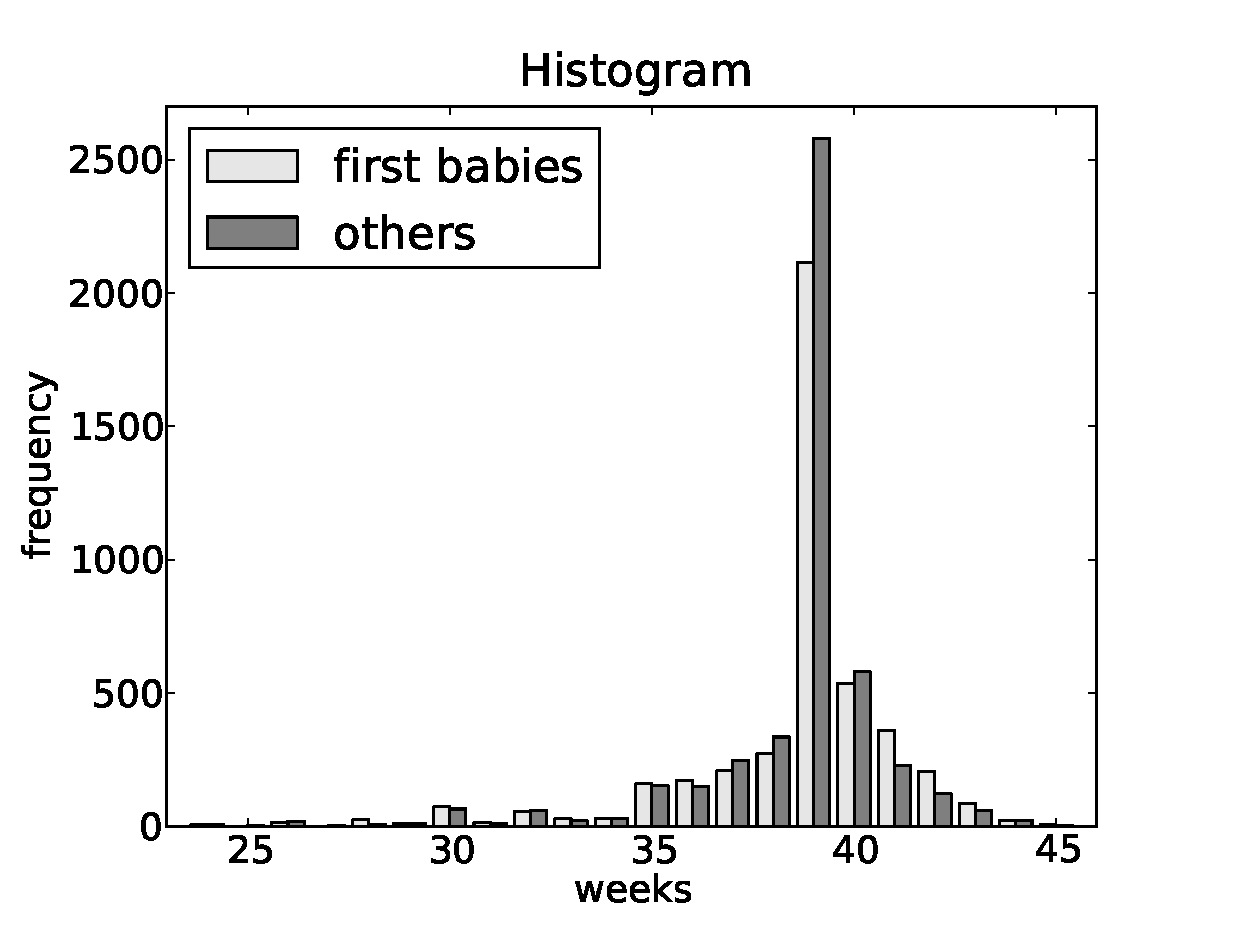
\includegraphics[height=2.5in]{workspace/nsfg_hist.eps}}
\caption{Histogram of pregnancy lengths.}
\label{nsfg_hist}
\end{figure}

Histograms are useful because they make the following features immediately
apparent:

\begin{description}

\item[Mode:] The most obvious feature of this distribution is the
  large frequency at 39 weeks.  The most common value in a
  distribution is called the {\bf mode}.  In this case, the mode is
  the summary statistic that does the best job of describing the
  typical value.

\item[Shape:] Around the mode, the distribution is asymmetric; it
  drops off quickly to the right and more slowly to the left.  From a
  medical point of view, this makes sense.  Babies are often born
  early, but seldom later than 42 weeks.  Also, the right side of the
  distribution is truncated because doctors often intervene after 42
  weeks.

\item[Outliers:] Values far from the mode are called {\bf outliers}.
  Some of these are just unusual cases, like babies born at 30 weeks.
  But many of them are probably due to errors, either in the reporting
  or recording of data.

\end{description}

Although histograms make some features apparent, they are usually not
useful for comparing two distributions.  In this example, there are
fewer ``first babies'' than ``others,'' so some of the apparent
differences in the histograms are due to sample sizes.


\section{Plotting PMFs}

We can solve that problem by normalizing the distributions---that
is, dividing through by the sample sizes---to generate the PMFs.
Figure~\ref{nsfg_pmf} shows the result.

\begin{figure}
% descriptive.py
\centerline{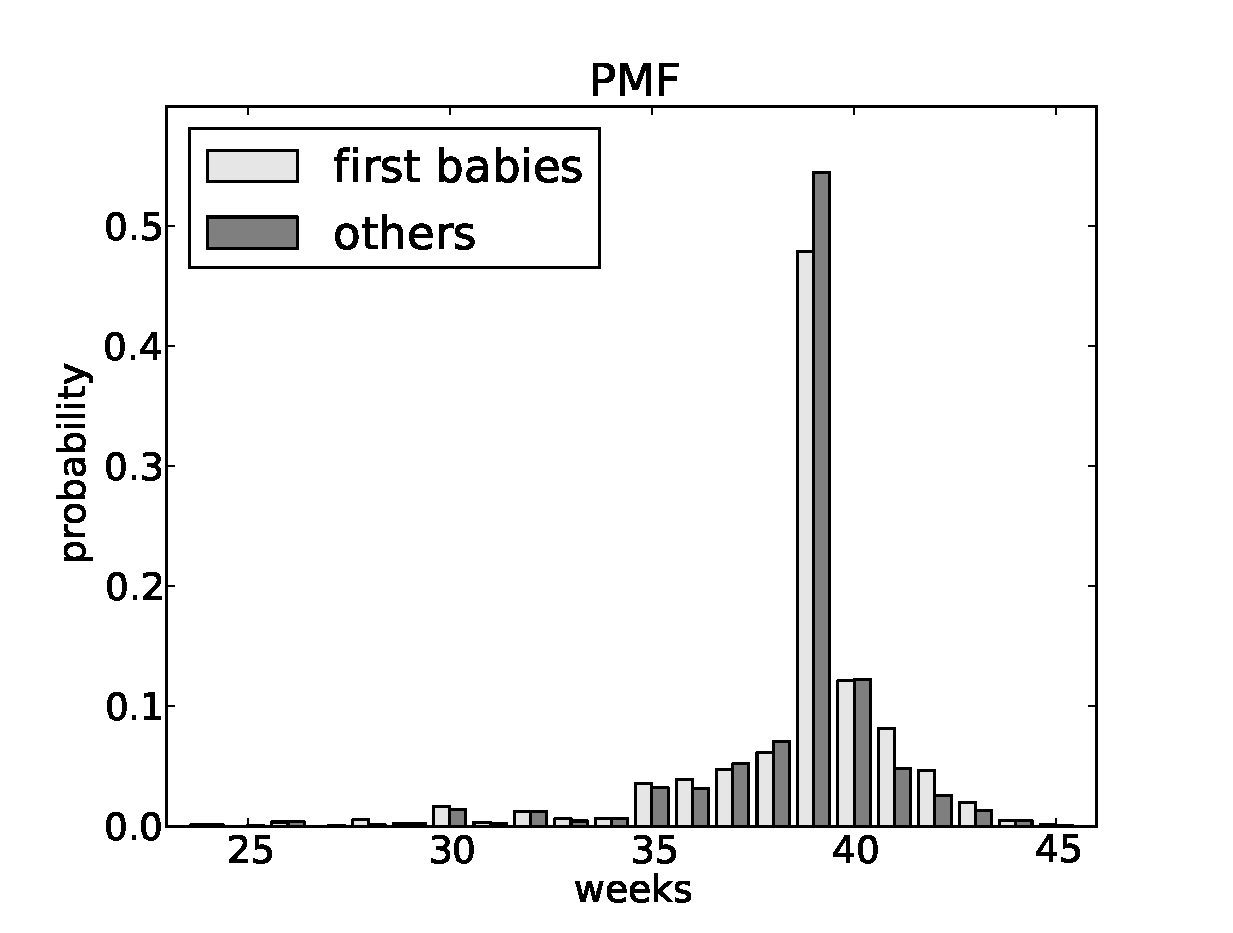
\includegraphics[height=2.5in]{workspace/nsfg_pmf.eps}}
\caption{PMF of pregnancy lengths.}
\label{nsfg_pmf}
\end{figure}

Using the PMF, we can see more clearly where the distributions
differ.  First babies seem to be less likely to arrive on time
(week 39) and more likely to be a little late (weeks 41 and 42).

\begin{ex}

Create a file named {\tt plot.py} and write a function called {\tt
  Hist} that takes a Hist object and generates a bar chart using {\tt
  pyplot.bar}.  This function should also work for Pmf objects.

Write another function called {\tt Hists} that takes two Hists (or
Pmfs) and generates side-by-side histograms like the figures in this
section.  You will have to read the {\tt pyplot} documentation to
adjust the width and position of the bars.

Use the data from the NSFG to generate plots like the ones in this
section.
\end{ex}


\section{Outliers}

Outliers are values that are far from the mode.  Outliers might
be caused by errors in collecting or processing the data, or
they might be legitimate, if unusual, measurements.

It is always a good idea to check for outliers, and sometimes
it is useful, and appropriate, to discard them.

In the list of pregnancy lengths for live births, the 10 lowest values are

\begin{verbatim}
weeks  count
0      1
4      1
9      1
13     1
17     2
18     1
19     1
20     1
21     2
22     7
\end{verbatim}

Values below 20 weeks are certainly errors, and values higher than 30
weeks are probably legitimate.  But there are several values in
between that are hard to interpret.

On the other end, the 10 highest values are

\begin{verbatim}
weeks  count
40     1116
41     587
42     328
43     148
44     46
45     10
46     1
47     1
48     7
50     2
\end{verbatim}

Again, there are some values here that are almost certainly errors, but
it is hard to know for sure.

Trimmed mean and variance.

Don't get carried away.


\section{Other visualizations}

Histograms and PMFs are useful for exploratory data analysis;
once you have an idea what is going on, it is often useful to
design a visualization that focuses on the apparent effect.

In the NSFG data, the biggest differences in the distributions are
near the mode.  So it makes sense to zoom in on that part of the
graph, and to transform the data to emphasize differences.

Figure~\ref{nsfg_diffs} shows the difference between the PMFs for weeks
35-45.  I multiplied by 100 to express the differences in percentage
points.

\begin{figure}
% ???
\centerline{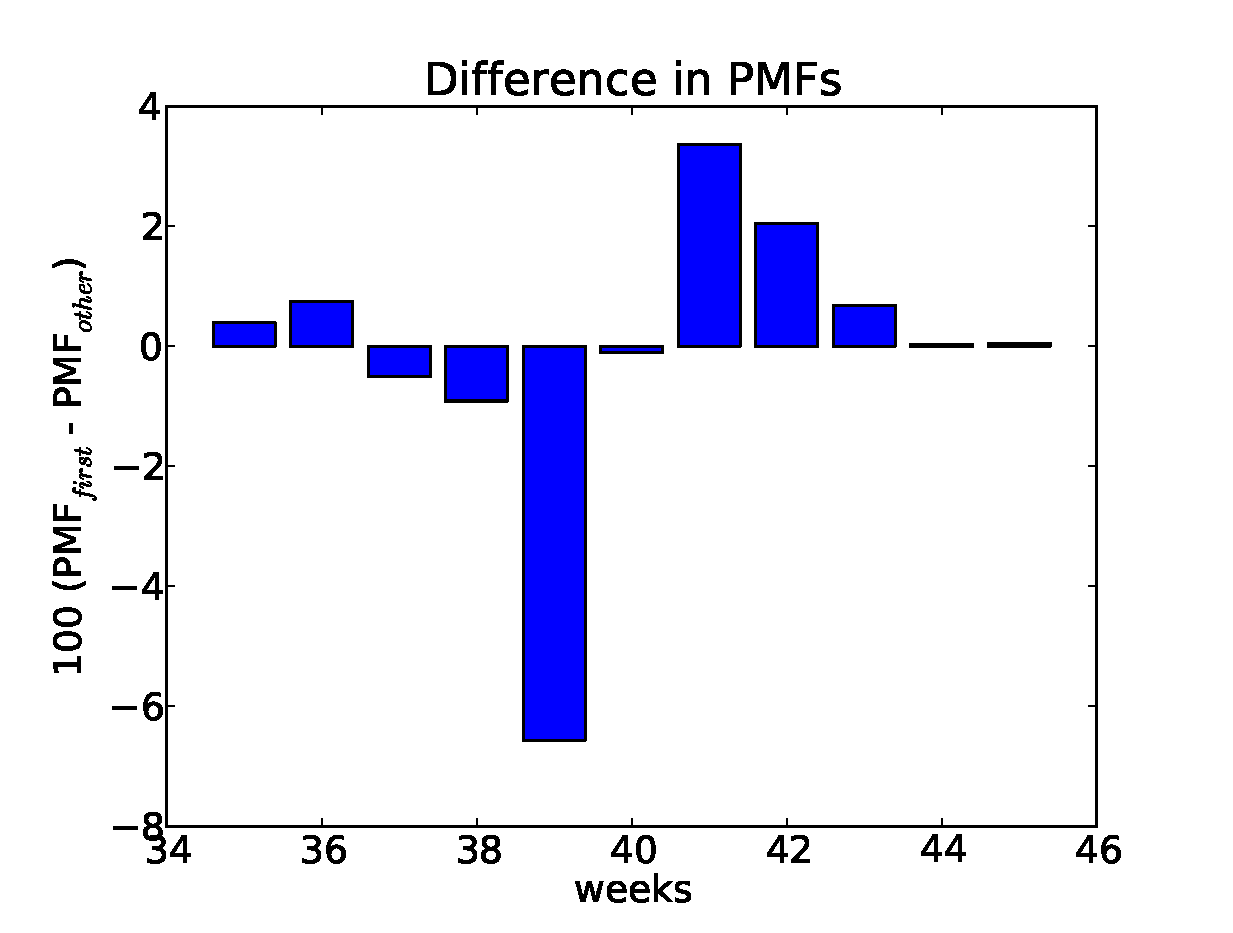
\includegraphics[height=2.5in]{workspace/nsfg_diffs.eps}}
\caption{Difference in percentage, by week.}
\label{nsfg_diffs}
\end{figure}

This figure makes the pattern clearer: first babies are
less likely to be born in week 39, and somewhat more likely
to be born in weeks 41 and 42.


\section{Relative risk}
\label{relative.risk}

We started with the question, ``Do first babies arrive late?''  To
make that more precise, let's say that a baby is early if it is born
during Week 37 or earlier, on time if it is born during Week 38, 39 or
40, and late if it is born during Week 41 or later.  Ranges like these
that are used to group data are called {\bf bins}.

\begin{ex}

Create a file named {\tt risk.py}.
Write functions named {\tt ProbEarly}, {\tt ProbOnTime} and
{\tt ProbLate} that take a PMF and compute the fraction of births
that fall into each bin.  Hint: write a generalized function
that these functions call.

Make three PMFs, one for first babies, one for others, and one for
all live births.  For each PMF, compute the probability of being
born early, on time, or late.

One way to summarize data like this is with a {\bf relative risk},
which is a ratio of two probabilities.  For example, the probability
that a first baby is born early is 18.2\%.  For other babies it is
16.8\%, so the relative risk is 1.08.  That means that first babies
are about 8\% more likely to be early.

Write code to confirm that result, then compute the relative risks of
being born on time and being late.

\end{ex}


\section{Conditional probability}

Imagine that someone you know is pregnant, and it is the beginning of
Week 39.  What is the chance that the baby will be born in the next
week?  How much does the answer change if it's a first baby?

We can answer these questions by computing a {\bf conditional
probability}, which is (ahem!) a probability that depends on a condition.
In this case, the condition is that we know the baby didn't arrive
during Weeks 0--38.

Here's one way to do it:

\begin{enumerate}

\item Given a PMF, generate a fake cohort of 1000 pregnancies.
For each number of weeks, $x$, the number of pregnancies with
duration $x$ is $1000 PMF(x)$.

\item Remove from the cohort all pregnancies with length less than 39.

\item Compute the PMF of the remaining durations; the result is the
conditional PMF.

\item Evaluate the conditional PMF at $x = 39$ weeks.

\end{enumerate}

\begin{ex}
Create a file named {\tt conditional.py}.
Write a program that implements this algorithm and computes the
probability that a baby will be born during Week 39, given that
it was not born prior to Week 39.

Generalize this program to compute the
probability that a baby will be born during Week $x$, given that
it was not born prior to Week $x$, for all $x$.

Plot this value as a function of $x$ for first babies and others.

\end{ex}


\section{Reporting results}

At this point we have explored the data and seen several apparent
effects.  For now, let's assume that these effects are real (but let's
remember that it is an assumption).  How should we report these
results?

The answer might depend on who is asking the question.  For example,
a scientist might be interested in any (real) effect, no matter how
small.  A doctor might only care about effects that are
{\bf clinically significant}; that is, differences that make a difference.
A pregnant woman might be interested in results that are relevant to
her, like the conditional probabilities in the previous section.

How you report results might also depend on your goals.  If you are
trying to demonstrate the significance of an effect, you might choose
summary statistics, like relative risk, that emphasize differences.
If you are trying to reassure a patient, you might choose statistics
that put the differences in context.

\begin{ex}

Based on the results from the previous exercises, suppose you were
asked to summarize what you learned about whether first
babies arrive late.

Which summary statistics would you use if you wanted to get a story
on the evening news?  Which ones would you use if you wanted to
reassure an anxious patient?

Finally, imagine that you are Cecil Adams, author of {\it The Straight
  Dope} (\url{straightdope.com}), and your job is to answer the
question, ``Do first babies arrive late?''  Write a paragraph that
uses your results to answer this question clearly, precisely, and
accurately.

\end{ex}


\section{Mean and variance of PMFs}

In Section~\ref{mean} we computed the mean of a sample by adding up
the elements and dividing by $n$.  If you are given a PMF, you can
still compute the mean, but the process is slightly different:

\[ \mu = \sum_i p_i x_i \]

where the $x_i$ are the unique values in the PMF and $p_i = PMF(x_i)$.
Similarly, you can compute variance like this:

\[ \sigma^2 = \sum_i p_i (x_i - mu)^2\]

\begin{ex}
In {\tt Pmf.py}, add methods named {\tt Mean} and {\tt Var} that compute
the mean and variance of a Pmf.

To test these methods, check that they are consistent with the
functions {\tt Mean} and {\tt Var} you wrote in {\tt thinkstats.py}.
\end{ex}


\section{The class size paradox}

At many American colleges and universities, the student-to-faculty
ratio is about 10:1.  But students are often surprised to discover
that their average class size is (much) bigger than 10.  There
are two reasons for the discrepancy:

\begin{itemize}

\item Students typically take 4--5 classes per semester, but
professors often teach 1 or 2.

\item The number of students who enjoy a small class is small,
but the number of students in a large class is...wait for it...large.

\end{itemize}

The first effect is obvious (at least once it is pointed out);
the second is more subtle.  So let's look at an example.  Suppose
that a college offers 65 classes in a given semester, with the
following distribution of sizes:

\begin{verbatim}
Sizes        Count
-----        -----
 0- 4          0
 5- 9          8
10-14          8
15-19         14
20-24          4
25-29          6
30-34         12
35-39          8
40-44          3
45-49          2
\end{verbatim}

If you ask the Dean for the average class size, he would
construct a PMF, compute the mean, and report that the
average class size is 24.

But if you survey a group of students, ask them how many
students are in their classes, and compute the mean, you would
conclude that the average class size is 29.

\begin{ex}
Build a PMF of these data and compute the mean.  Now compute the
average class size as perceived by students.

Note: since the data have been grouped in bins, you can use the
mid-point of each bin.
\end{ex}


\section{Glossary}

\begin{description}

\item[central tendency:] A characteristic of a sample or population;
intuitively, it is the most average value. 

\item[spread:] A characteristic of a sample or population;
intuitively, it describes how much variability there is.

\item[variance:] A summary statistic often used to quantify spread.

\item[standard deviation:] The square root of variance, also used
as a measure of spread.

\item[frequency:] The number of times a value appears in a sample.

\item[histogram:] A mapping from values to frequencies, or a graph
that shows this mapping.

\item[probability:] A frequency expressed as a fraction of the sample
size.

\item[normalization:] The process of dividing a frequency by a sample
size to get a probability.

\item[distribution:] A summary of the values that appear in a sample
and the frequency, or probability, of each.

\item[pmf:] Probability mass function: a representation of a distribution
as a function that maps from values to probabilities.

\item[mode:] The most frequent value in a sample.

\item[outlier:] A value far from the central tendency.

\item[bin:] A range used to group nearby values.

\item[relative risk:] A ratio of two probabilities, often used to measure
a difference between distributions.

\item[conditional probability:] A probability computed under the assumption
that some condition holds.

\item[clinically significant:] A result, like a difference between groups,
that is relevant in (often medical) practice.

\end{description}


\chapter{Cumulative distribution functions}
\label{cumulative}

\section{The limits of PMFs}

PMFs work well if the number of different values is less than
about 50.  But as the number of values increases, the probability
associated with each value gets smaller and the effect of random noise
increases.

For example, we might be interested in the distribution of birth
weights.  In the NSFG, the integer variables \verb"birthwgt_lb" and
\verb"birthwgt_oz" encode birth weight in pounds and ounces.
Figure~\ref{nsfg_birthwgt_pmf} shows the PMF of these values,
converted to total weight in ounces, for first babies and others.

\begin{figure}
% cumulative.py
\centerline{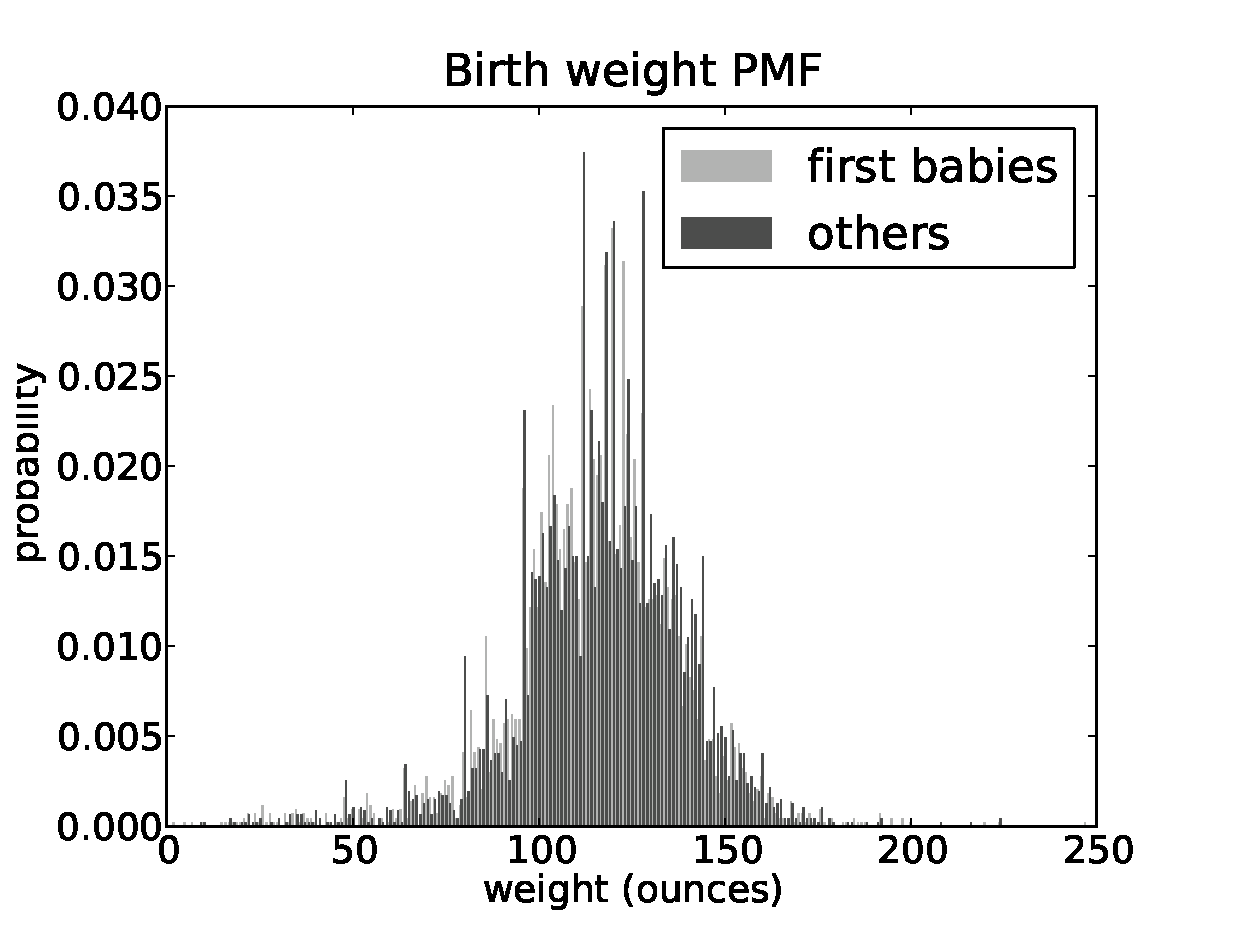
\includegraphics[height=2.5in]{workspace/nsfg_birthwgt_pmf.eps}}
\caption{PMF of birth weights.}
\label{nsfg_birthwgt_pmf}
\end{figure}

Overall, these distributions resemble the familiar ``bell curve,'' with
many values near the mean and a few values much higher and lower.

But parts of this figure are hard to interpret.  There are many spikes
and valleys, and some apparent differences between the distributions.
It is hard to tell which of these features are significant.  Also, it
is hard to see overall patterns; for example, which distribution do
you think has the higher mean?

These problems can be mitigated by binning the data;
that is, dividing the domain into non-overlapping intervals and counting
the number of values in each bin.  Binning can be useful, but it is
tricky to get the size of the bins right.  If they are big enough to
smooth out noise, they might also smooth out useful information.

An alternative that avoids these problems is the {\bf cumulative
distribution function}, or {\bf CDF}.  But before we can get to that,
we have to talk about percentiles.


\section{Percentiles}

If you have taken a standardized test, you probably got your
results in the form of a raw score and a {\bf percentile rank}.
In this context, the percentile rank is the fraction of people who
scored lower than you (or the same).  So if you are ``in the 90th
percentile,'' you did as well as or better than 90\% of the people who
took the exam.

Here's how you could compute the percentile rank of a value,
\verb"your_score", relative to the scores in the sequence {\tt
  scores}:

\begin{verbatim}
def PercentileRank(scores, your_score):
    count = 0
    for score in scores:
        if score <= your_score:
            count += 1

    percentile_rank = 100.0 * count / len(scores)
    return percentile_rank
\end{verbatim}
%
% see score_example.py
%
For example, if the scores in the sequence were 55, 66, 77, 88 and 99,
and you got the 88, then your percentile rank would be {\tt 100 * 4 / 5}
which is 80.

If you are given a value, it is easy to find its percentile rank; going
the other way is slightly harder.  If you are given a percentile rank
and you want to find the corresponding value, one option is to
sort the values and search for the one you want:

\begin{verbatim}
def Percentile(scores, percentile_rank):
    scores.sort()
    for score in scores:
        if PercentileRank(scores, score) >= percentile_rank:
            return score
\end{verbatim}

The result of this calculation is a {\bf percentile}.  For example,
the 50th percentile is the value with percentile rank 50.  In the
distribution of exam scores, the 50th percentile is 77.

\begin{ex}
This implementation of {\tt Percentile} is not very efficient.  A
better approach is to use the percentile rank to compute the index of
the corresponding percentile.  Write a version of {\tt Percentile} that
uses this algorithm.
\end{ex}

\begin{ex}
This exercise is optional.

If you only want to compute one percentile, it is not efficient
to sort the scores.  A better option is the selection algorithm,
which you can read about at \url{wikipedia.org/wiki/Selection_algorithm}.

Write (or find) an implementation of the selection algorithm and use
it to write an efficient version of {\tt Percentile}.
\end{ex}


\section{Cumulative distribution functions}

Now that we understand percentiles, we are ready to tackle the
cumulative distribution function (CDF).  The CDF is the function that
maps values to their percentile rank in a distribution.

The CDF is a function of $x$, where $x$ is any value that might appear
in the distribution.  To evaluate $CDF(x)$ for a particular value of
$x$, we compute the fraction of the values in the sample less than (or
equal to) $x$.

Here's what that looks like as a Python function that takes a sample,
{\tt t}, and a value, {\tt x}:

\begin{verbatim}
def Cdf(t, x):
    count = 0.0
    for value in t:
        if value <= x:
            count += 1.0

    prob = count / len(t)
    return prob
\end{verbatim}

This function should look familiar; it is almost identical to {\tt
  PercentileRank}, except that the result is in a probability in the
range 0--1 rather than a percentile rank in the range 0--100.

As an example, suppose a sample has the values $\{1, 2, 2, 3, 5\}$.
Here are some values from its CDF:

\begin{eqnarray*}
CDF(0) &=& 0    \\
CDF(1) &=& 0.2    \\
CDF(2) &=& 0.6    \\
CDF(3) &=& 0.8    \\
CDF(4) &=& 0.8    \\
CDF(5) &=& 1    \\
\end{eqnarray*}
%
We can evaluate the CDF for any value of $x$, not just
values that appear in the sample.
If $x$ is less than the smallest value in the sample, $CDF(x)$ is 0.
If $x$ is greater than the largest value, $CDF(x)$ is 1.

Figure~\ref{example_cdf} is a graphical representation of this CDF.

\begin{figure}
% Cdf_test.py
\centerline{\includegraphics[height=2.5in]{workspace/example_cdf.eps}}
\caption{Example of a CDF.}
\label{example_cdf}
\end{figure}

The CDF of a sample is a step function.  In the next chapter we
will see distributions whose CDFs are continuous functions.  

The function {\tt Cdf}, above, is efficient enough if we only want
to evaluate the CDF at one point.  But there are several operations
we might want to perform on CDFs:

\begin{description}

\item[Evaluate:] Given a value $x$, evaluate $CDF(x)$ to get a
  probability $p$.  This operation computes percentile ranks.

\item[Invert:] Given a probability $p$, find the value $x$ so that
  $CDF(x) = p$.  This operation computes percentiles.

\item[Render:] Generate a sequence of points suitable for plotting the
  CDF.

\end{description}

It is not obvious what data structures we should use to implement
these operations; there are several reasonable choices.  In the
following exercise I recommend an option that is simple and efficient.

\begin{ex}
Create a file named {\tt Cdf.py} and write a definition for a class
named {\tt Cdf} that represents a CDF.  The attributes of a Cdf
object are {\tt xs}, which is a sorted list of the unique values
in the sample, and {\tt ps} which is a list of probabilities.

Write a simple constructor that takes {\tt xs} and {\tt ps} as
parameters, then write two functions:

\begin{description}

\item[{\tt MakeCdfFromDict}]: Takes a dictionary that maps from
values to frequencies, computes {\tt xs} and {\tt ps}, and returns
a {\tt Cdf} object.

\item[{\tt MakeCdfFromList}]: Takes a sequence of values, makes
a dictionary that maps from values to frequencies, and uses
{\tt MakeCdfFromDict} to make and return a {\tt Cdf} object.

\end{description}

Now write the following methods for {\tt Cdf}:

\begin{description}

\item[{\tt Prob}]: Given a value $x$, compute the probability $p = CDF(x)$.

\item[{\tt Value}]: Given a probability $p$, compute the
corresponding value, $x$; that is, the inverse CDF of $p$.

\item[{\tt Render}]: Return two lists, {\tt xs} and {\tt ps}, suitable
for plotting the CDF.  Notice that the CDF is a step function, so these
lists should have two elements for each unique value in the distribution.

\end{description}

Test your code by computing the CDF of the values $\{1, 2, 2, 3, 5\}$.
Test {\tt Prob} and {\tt Value} using the examples in this section.

Write a function that plots the CDF with the {\tt pyplot} function
{\tt plot}.  Confirm that your plot looks like the figure above.

You can download a solution from \url{thinkstatsbook.com/Cdf.py}.
\end{ex}


\section{Back to the survey data}

Figure~\ref{nsfg_birthwgt_cdf} shows the CDFs of birth weight for
first babies and others in the NSFG dataset.

\begin{figure}
% cumulative.py
\centerline{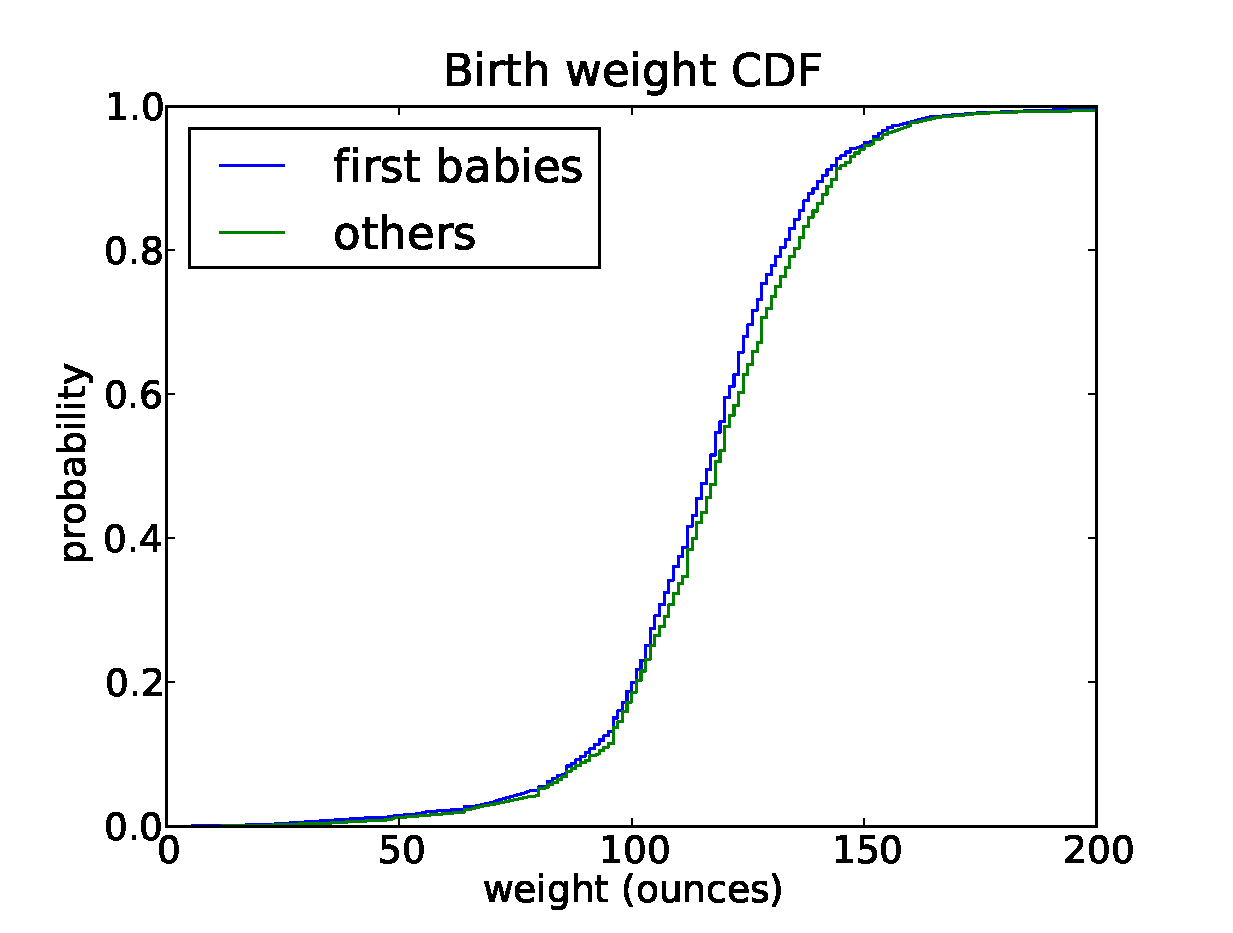
\includegraphics[height=2.5in]{workspace/nsfg_birthwgt_cdf.eps}}
\caption{CDF of birth weights.}
\label{nsfg_birthwgt_cdf}
\end{figure}

This figure makes the shape of the distributions, and the differences
between them, much clearer.  We can see that first babies are slightly
lighter throughout the distribution, with a larger discrepancy above 
the mean.

\begin{ex}
This exercise is optional.  In the figure above, you might notice
a sequence of equally-spaced values with higher frequency than
their neighbors.  See if you can figure out what it going on.
Hint: look at the PMF of \verb"birthwgt_oz".
\end{ex}

\begin{ex}
How much did you weigh at birth?  If you don't know, call your mother
or someone else who knows.  Using the pooled data (all live births),
compute the distribution of birth weights and use it to find your
percentile rank.  If you were a first baby, find your percentile rank
in the distribution for first babies.  Otherwise use the distribution
for others.  How big is the difference between your percentile ranks
in the two distributions?
\end{ex}

\begin{ex}
Suppose you and your classmates compute the percentile rank of your
birth weights and then compute the CDF of the percentile ranks.  What do
you expect it to look like?
\end{ex}


\section{Conditional distributions}

A {\bf conditional distribution} is the distribution of a subset of
the data which is selected according to a condition.

For example, if you are above average in weight, but way above average
in height, then you might be relatively light for your height.  Here's
how you could make that claim more precise.

\begin{enumerate}

\item Select a cohort of people who are the same height as you (within
some range).

\item Find the CDF of weight for those people.

\item Find the rank percentile of your weight in that distribution.

\end{enumerate}


\begin{ex}
Find out how tall (long, actually) you were at birth.  If you don't
know, call your mother again.  Find the CDF of birth weight for
people who were the same height, and compute your percentile rank
in that CDF.

Now find the rank percentile of your height conditioned on your weight.
\end{ex}


\section{Age group ranking}

Percentile ranks are useful for comparing measurements from different
tests, or tests applied to different groups.

For example, people who compete in foot races are usually grouped by
age and gender.  To compare people in different groups, you can convert
race times to percentile ranks.

\begin{ex}

I recently ran in the 27th Anniversary Edition James Joyce Ramble 10K
in Dedham MA.  The results are available from
\url{coolrunning.com/results/10/ma/Apr25_27thAn_set1.shtml}.
Go to that page and find my results.  I came in 97th in a field
of 1633, so what is my percentile rank in the field?

In my division (M4049 means ``male between 40 and 49 years of age'')
I came in 26th out of 256.  What is my percentile rank in my division?
What does that tell you about my division?

If I am still running in 10 years (and I hope I am), I will be in
the M5059 division.  Assuming that my percentile rank in my division
is the same, how much slower should I expect to be?

I maintain a friendly rivalry with a student of mine who is in the
F2039 division.  How fast does she have to run her next 10K to
``beat'' me in terms of percentile ranks?

\end{ex}

\section{Random numbers}

CDFs are also useful for generating random numbers
with a given distribution.  Here's how:

\begin{itemize}

\item Choose a random probability in the range 0--1.

\item Use {\tt Cdf.Value} to find the value in the distribution
that corresponds to the probability you chose.

\end{itemize}

It might not be obvious why this works, but since it is easier
to implement than explain, let's try it out.

\begin{ex}

Add a method to the Cdf class, called {\tt Sample}, that takes
an integer {\tt n} and returns a list of $n$ values chosen at
random from the distribution.  Hint: use {\tt random.random}.

Using the distribution of birth weights from the NSFG, generate a
random sample with 1000 elements.  Compute the CDF of the sample.
Make a plot that shows the original CDF and the CDF of the random
sample.  For large values of $n$, the distributions should be
the same.

\end{ex}

This process, generating a random sample based on a measured sample,
is called {\bf resampling}.


\section{Summary statistics revisited}

Once you have computed a CDF, it is easy to compute other summary
statistics.  The median is just the 50th percentile\footnote{You might
see other definitions of the median.  In particular,
some sources suggest that if you have an even number of elements in
a sample, the median is the average of the middle two elements.
This is an unnecessary special case, and it has the odd effect of
generating a value that is not in the sample.  As far
as I'm concerned, the median is the 50th percentile.  Period.}.
The 25th and 75th percentiles are often used to check whether
a distribution is symmetric, and their difference, which is called
the {\bf interquartile range} measures the spread.

\begin{ex}
Compute the 25th, 50th, and 75th percentiles of the birth weight
CDF.  Do these values suggest that the distribution is symmetric?

Int {\tt Cdf}, add a method called {\tt Median} that computes the
median, and one called {\tt Interquartile} that computes
the interquartile range.
\end{ex}


\section{Glossary}

\begin{description}

\item[percentile rank:] The percentage of values in a distribution that are
less than or equal to a given value.

\item[CDF:] A function that maps from values to their percentile ranks.

\item[percentile:] The value associated with a given percentile rank.

\item[conditional distribution:] A distribution computed under the assumption
that some condition holds.

\item[resampling:] The process of generating a random sample from a
distribution that was computed from a sample.

\end{description}



\chapter{Continuous distributions}
\label{continuous}

The distributions we have used so far are called {\bf
  empirical distributions} because they are based on empirical
observations.

The alternative is a {\bf continuous distribution}, which is
characterized by a CDF that is a continuous function (as opposed to a
step function).  Many real world phenomena can be approximated by
continuous distributions, which is why they are useful.

\section{The exponential distribution}

I'll start with the exponential distribution because it is
easy to work with.  In the real world, exponential distributions
come up when we look at a series of events and measure the
times between events, which are called {\bf interarrival times}.
If the events are equally likely to occur at any time, the distribution
of interarrival times tends to look like an exponential distribution.

The CDF of the exponential distribution is:

\[ CDF(x) = 1 - e^{-\lambda x} \]

The parameter, $\lambda$, determines the shape of the
distribution.  Figure~\ref{expo_cdf} shows what this CDF looks like with
$\lambda = 2$.

\begin{figure}
\centerline{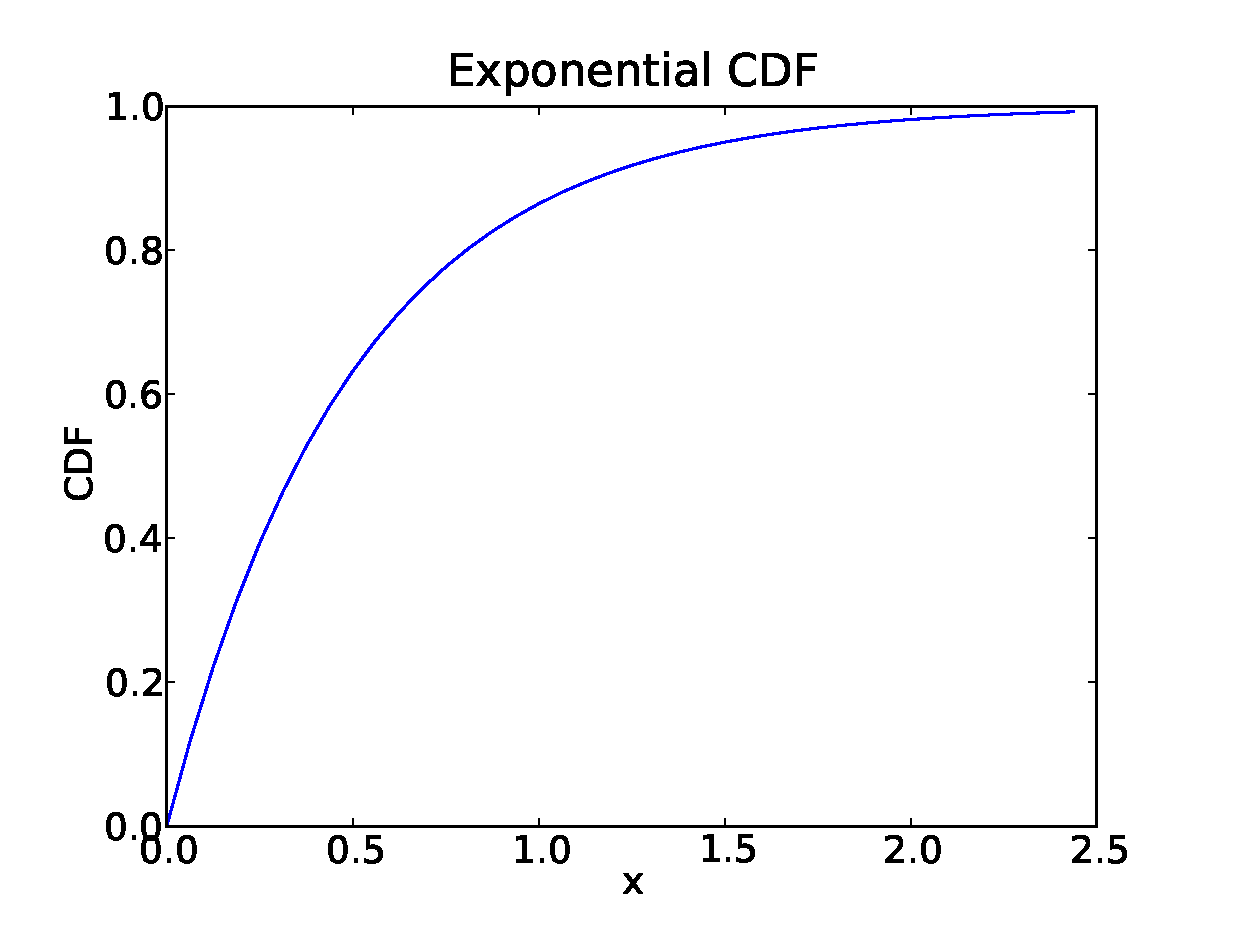
\includegraphics[height=2.5in]{workspace/expo_cdf.eps}}
\caption{CDF of exponential distribution.}
\label{expo_cdf}
\end{figure}

In general, the mean of an exponential distribution is $1 / \lambda$,
so the mean of this distribution is 0.5.  The median is $log(2) / \lambda$,
which is roughly 0.35.

To see an example of a distribution that is approximately exponential,
we will look at the interarrival time of babies.
On December 18, 1997, 44 babies were born in a hospital in Brisbane,
Australia\footnote{This example is based on information and data from
  Dunn, ``A Simple Dataset for Demonstrating Common Distributions,''
  Journal of Statistics Education v.7, n.3 (1999).}.  The times of
birth for all 44 babies were reported in the local paper; you can
download the data from \url{thinkstatsbook.com/babyboom.dat}.

Figure~\ref{interarrivals} shows the CDF of the interarrival times
in minutes.  It seems to have the general shape of an exponential
distribution, but how can we tell?

\begin{figure}
\centerline{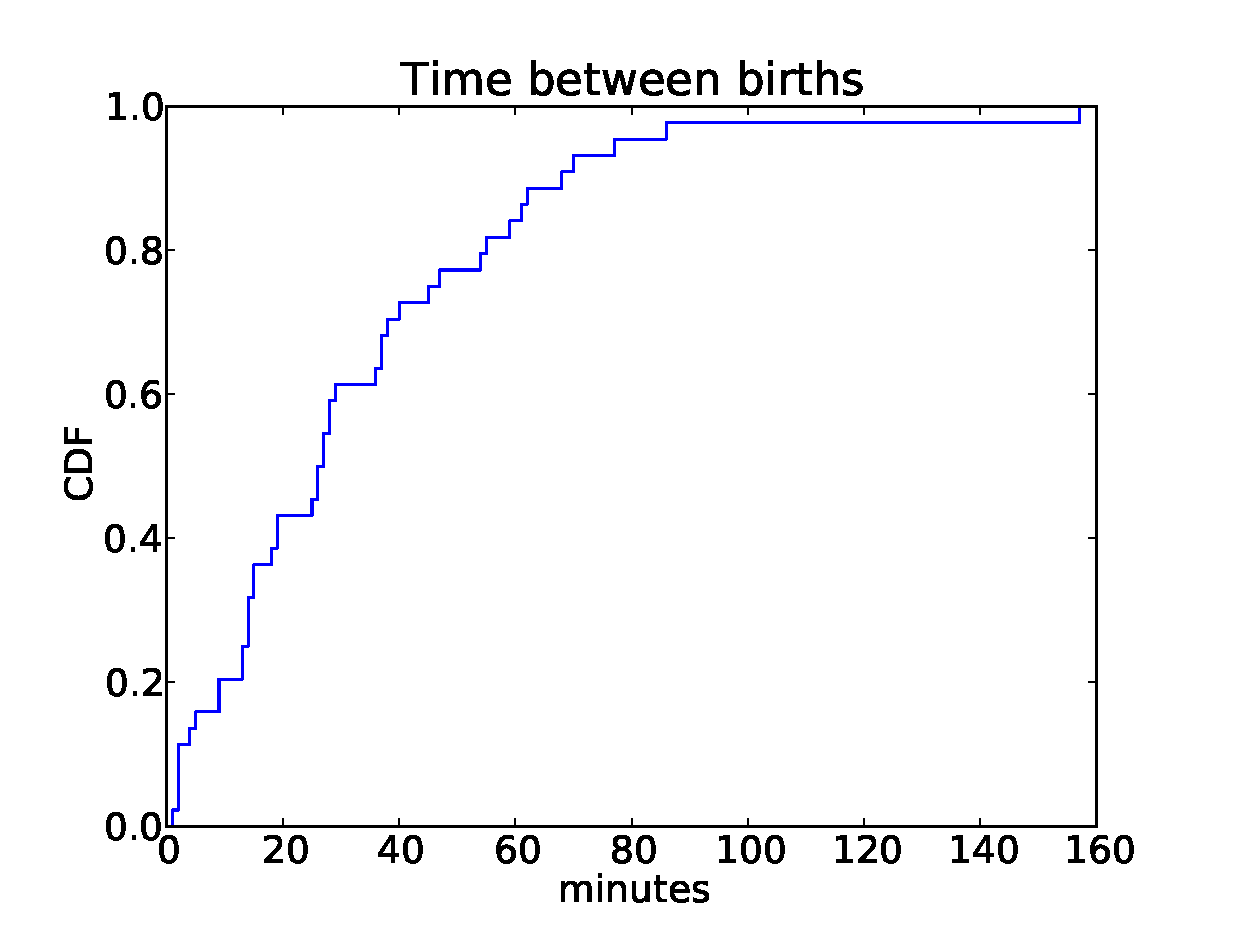
\includegraphics[height=2.5in]{workspace/interarrivals.eps}}
\caption{Interarrival times.}
\label{interarrivals}
\end{figure}

One way is to plot the complementary CDF, $1 - CDF(x)$, on a
log-$y$ scale.  For data from an exponential distribution, the result
is a straight line.  Let's see why that works...

If you plot the complementary CDF (CCDF) of a dataset that you think is
exponential, you expect to see a function like:

\[ y = \sim e^{-\lambda x} \]

If you take the log of both sides of this equation, you get:

\[ \log y \sim -\lambda x \]

So on a log-$y$ scale the CCDF is a straight line
with slope $-\lambda$.

Figure~\ref{interarrivals_logy} shows the CCDF of the interarrivals on
a log-$y$ scale.  It is not exactly straight, which suggests that the
exponential distribution is only an approximation.  Most likely the
underlying assumption---that a birth is equally likely at any time of
day---is not exactly true.

\begin{figure}
\centerline{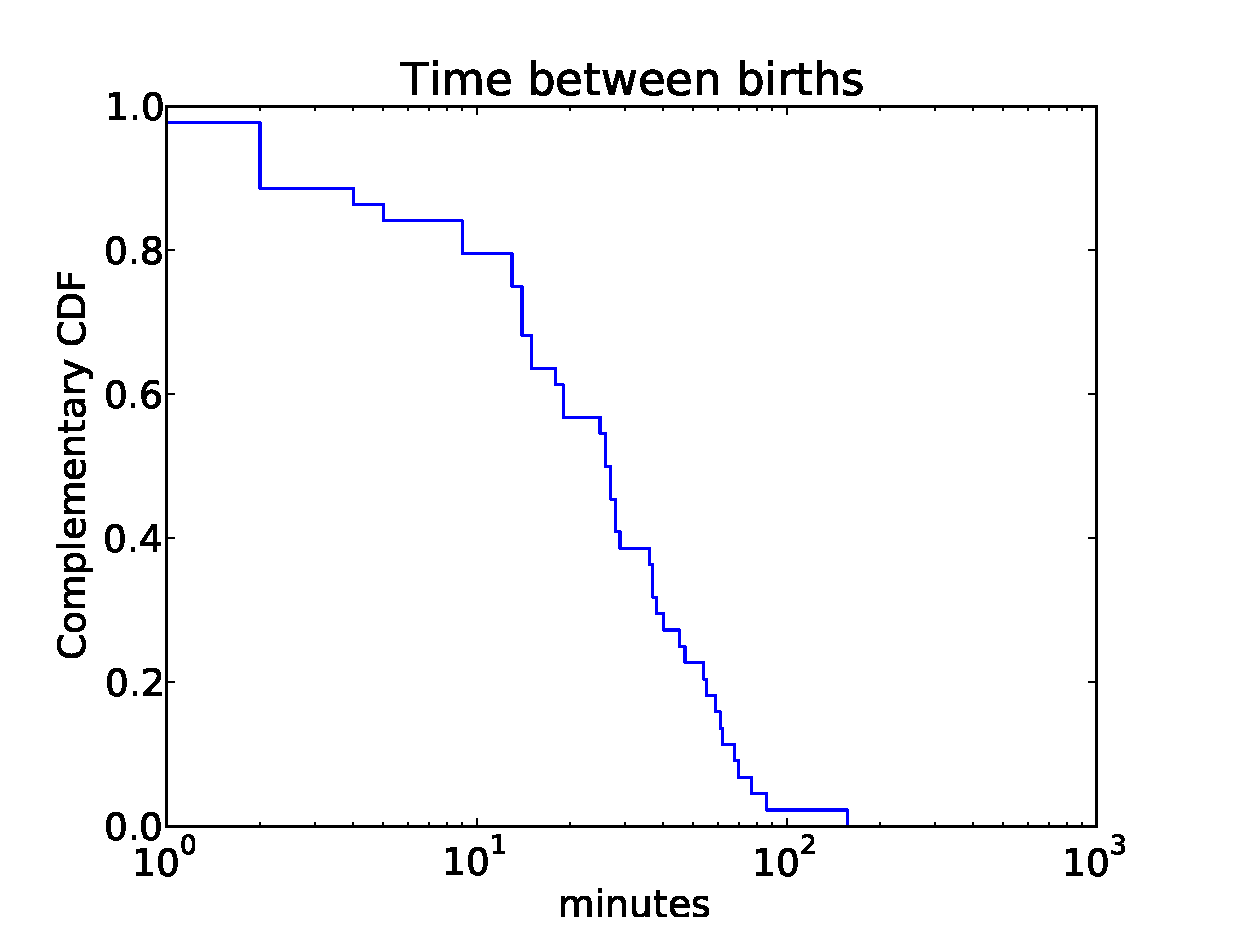
\includegraphics[height=2.5in]{workspace/interarrivals_logy.eps}}
\caption{Interarrival times.}
\label{interarrivals_logy}
\end{figure}

\begin{ex}
For small values of $n$, we don't expect an empirical distribution
to fit a continuous distribution exactly.  One way to evaluate
the quality of fit is to generate a sample from a continuous
distribution and see how well it matches the data.

The function {\tt expovariate} in the {\tt random} module
generates random values from an exponential distribution with
a given value of $\lambda$.

Use it to generate 44 values from an exponential distribution with
mean 32.6.  Plot the CCDF on a log-$y$ scale and compare
it to Figure~\ref{interarrivals_logy}.

Hint: use the function {\tt pyplot.yscale} to plot the $y$ axis
on a log scale.
\end{ex}

\begin{ex}
Most people don't know what time they were born, but most people know
their birthday.

Collect the birthdays of the students in your class, sort them, and
compute the interarrival times in days.  Plot the CDF of the interarrival
times and the CCDF on a log-$y$ scale.  Does it look like
an exponential distribution?
\end{ex}


\section{The Pareto distribution}

The Pareto distribution is named after the economist Vilfredo Pareto,
who used it to describe the distribution of wealth (see
\url{wikipedia.org/wiki/Pareto_distribution}).  Since then, people
have used it to describe a variety of phenomena in the natural and
social sciences, including sizes of cities and towns, sand particles
and meteorites, forest fires and earthquakes.

The Pareto distribution is characterized by the following CDF:

\[ CDF(x) = 1- \left( \frac{x}{x_m} \right) ^{-\alpha} \]

The parameters $x_m$ and $\alpha$ determine the location and shape of
the distribution.  $x_m$ is the minimum possibile value.
Figure~\ref{pareto_cdf} shows the CDF of a Pareto distribution with
parameters $x_m = 0.5$ and $\alpha = 1$.

\begin{figure}
\centerline{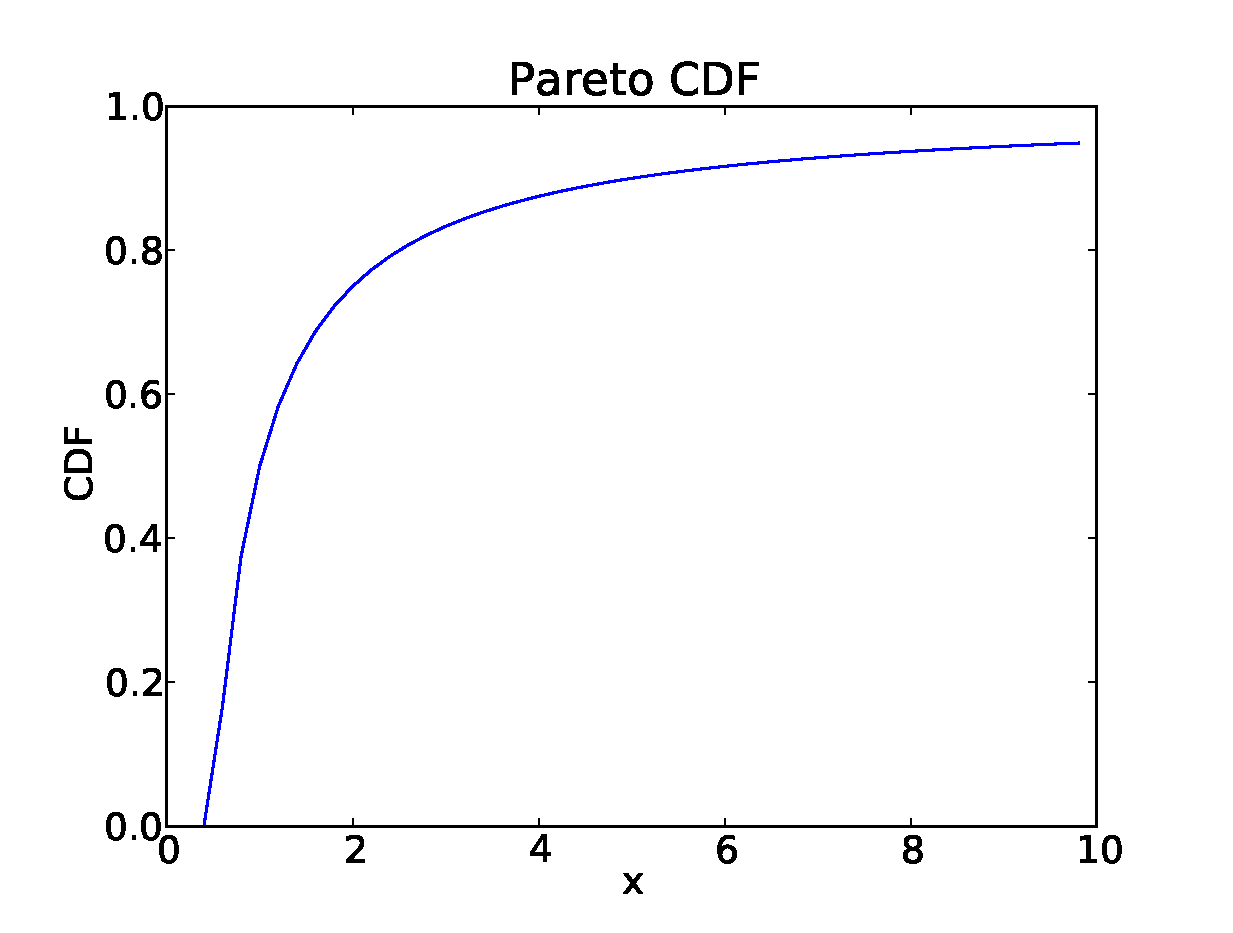
\includegraphics[height=2.5in]{workspace/pareto_cdf.eps}}
\caption{CDF of a Pareto distribution.}
\label{pareto_cdf}
\end{figure}

The median of this distribution is $x_m 2^{1/alpha} = 1$, but the
95th percentile is 10.  By contrast, the exponential distribution
with median 1 has 95th percentile of only 1.5.

There is a simple visual test that indicates whether an empirical
distribution is well-characterized by a Pareto distribution: on a
log-log scale, the CCDF looks like a straight line.  The derivation is
similar to what we saw in the previous section.

If you plot a the CCDF of a sample from a Pareto distibution on a
linear scale, you expect to see a function like:

\[ y \sim \left( \frac{x}{x_m} \right) ^{-\alpha} \]

Taking the log of both sides yields:

\[ \log y \sim -\alpha (\log x - \log x_m ) \]

So if you plot $\log y$ versus $\log x$, it should look like a
straight line with slope $-\alpha$ and intercept $-\alpha \log x_m$.

\begin{ex}

The {\tt random} module provides {\tt paretovariate},
which generates random values from a Pareto distribution.  It takes
a parameter for $\alpha$, but no parameter for $x_m$.  What is
the default value for $x_m$?

Write a wrapper function named {\tt paretovariate} that takes $\alpha$
and $x_m$ as parameters and uses {\tt random.paretovariate} to
generate values from a two-parameter Pareto distribution.

Use your function to generate a sample from a Pareto distribution.
Compute the CCDF and plot it on a log-log scale.  Is it a straight
line?  What is the slope?

\end{ex}

\begin{ex}
To get a feel for the Pareto distribution, imagine what the world
would be like if the distribution of human height were Pareto.
Choosing the parameters $x_m = 100$ cm and $\alpha = 1.7$, we
get a distribution with a reasonable minimum, 100 cm,
and median, 150 cm.

Generate 6 billion random values from this distribution.  What is the
mean of this sample?  What fraction of the population is shorter than
the mean?  How tall is the tallest person in Pareto World?

\end{ex}

\begin{ex}

Zipf's law is an observation about how often different words are used.
The most common words have very high frequencies, but there are many
unusual words, like ``hapaxlegomenon,'' that appear only a few times.
Zipf's law predicts that in a body of text, called a ``corpus,'' the
distribution of word frequencies is roughly Pareto.

Find a large corpus, in any language, in electronic
format.  Count how many times each word appears.  Find the CCDF of the
word counts and plot it on a log-log scale.  Does Zipf's law hold?
What is the value of $\alpha$, approximately?

\end{ex}

\begin{ex}

The Weibull distribution is a generalization of the exponential
distribution that comes up in failure analysis
(see \url{wikipedia.org/wiki/Weibull_distribution}).

Can you find a transformation that makes a Weibull distribution look
like a straight line?  What do the slope and intercept of the
line indicate?

Use {\tt random.weibullvariate} to generate a sample from a
Weibull distribution and use it to test your transformation.

\end{ex}




\section{The normal Distribution}

\newcommand{\erf}{\mathrm{erf}}

The normal distribution, also called Gaussian, is the most
commonly used because it describes so many phenomena, at least
approximately.  It turns out that there is a good reason for
its ubiquity, which we will get to soon.

The normal distribution has many properties that make it amenable for
analysis, but unfortunately the CDF is not one of them.  Unlike the
other distributions we have looked at, there is no closed-form
expression for the normal CDF; the most common alternative is to write
it in terms of a special function called the {\bf error function},
written $\erf$:

\[ erf(x) = \frac{2}{\sqrt{\pi}} \int_{-\infty}^x e^{-t^2} dt \]

\[ CDF(x) = \frac{1}{2} \left[ 1 +
  \erf \left( \frac{x - \mu}{\sigma \sqrt{2}} \right) \right] \]

The parameters $\mu$ and $\sigma$ determine the mean and standard
deviation of the distribution.

If these formulas make your eyes hurt, don't worry; they are
easy to implement in Python.  There are many fast and accurate ways
to approximate $\erf$.  You can download one of them from
\url{thinkstatsbook.com/erf.py}, which provides functions
named {\tt erf} and {\tt NormalCdf}.

Figure~\ref{normal_cdf} shows the CDF of the normal distribution
with parameters $\mu=2.0$ and $\sigma=0.5$.  The sigmoid shape of
this curve is a recognizable characteristic of a normal distribution.

\begin{figure}
\centerline{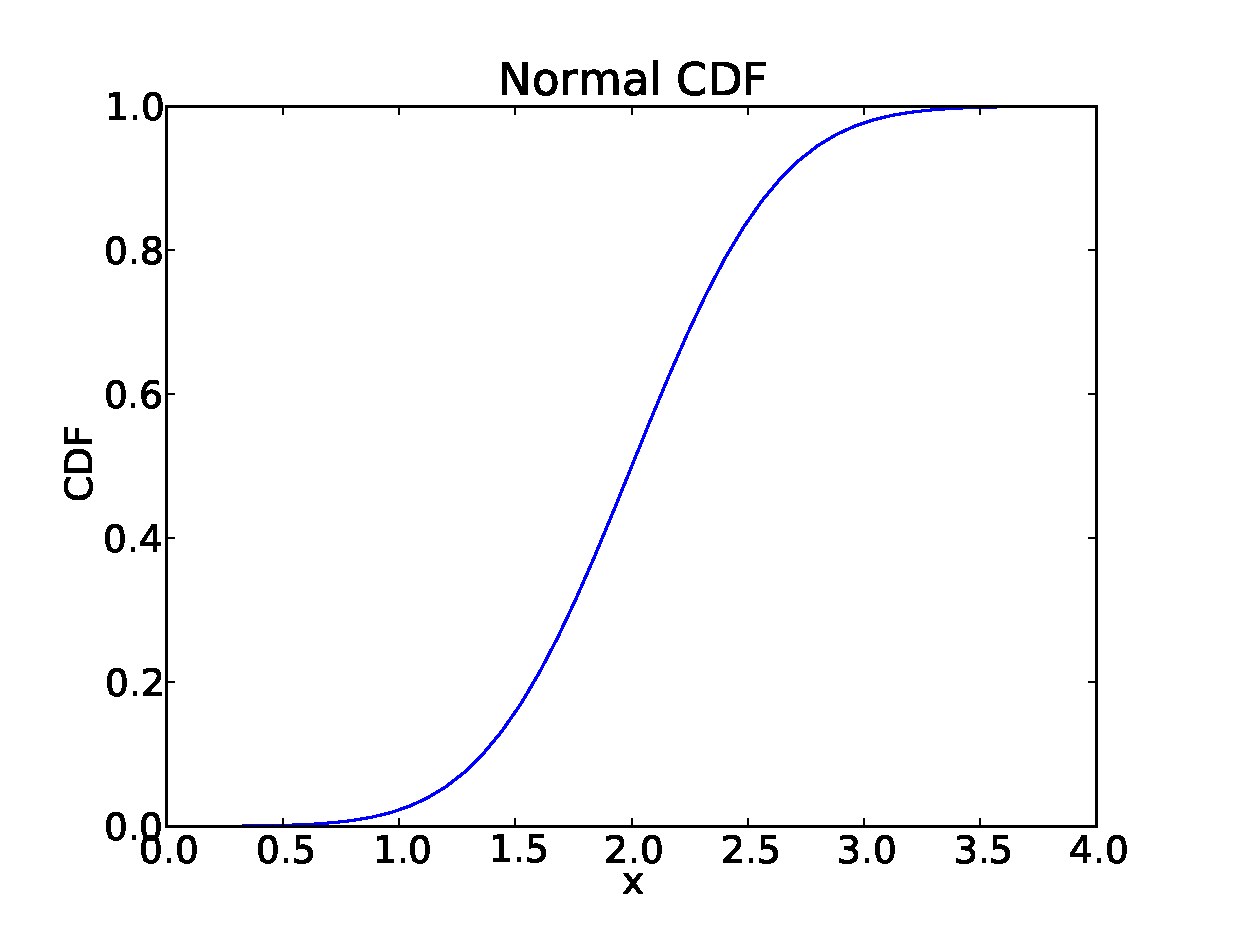
\includegraphics[height=2.5in]{workspace/normal_cdf.eps}}
\caption{CDF of a Normal distribution.}
\label{normal_cdf}
\end{figure}

In the previous chapter we looked at the distribution of birth
weights in the NSFG.  Figure~\ref{nsfg_birthwgt_model} shows the
empirical CDF of weights for all live births and the CDF of
a normal distribution with the same mean and variance.

\begin{figure}
% cumulative.py
\centerline{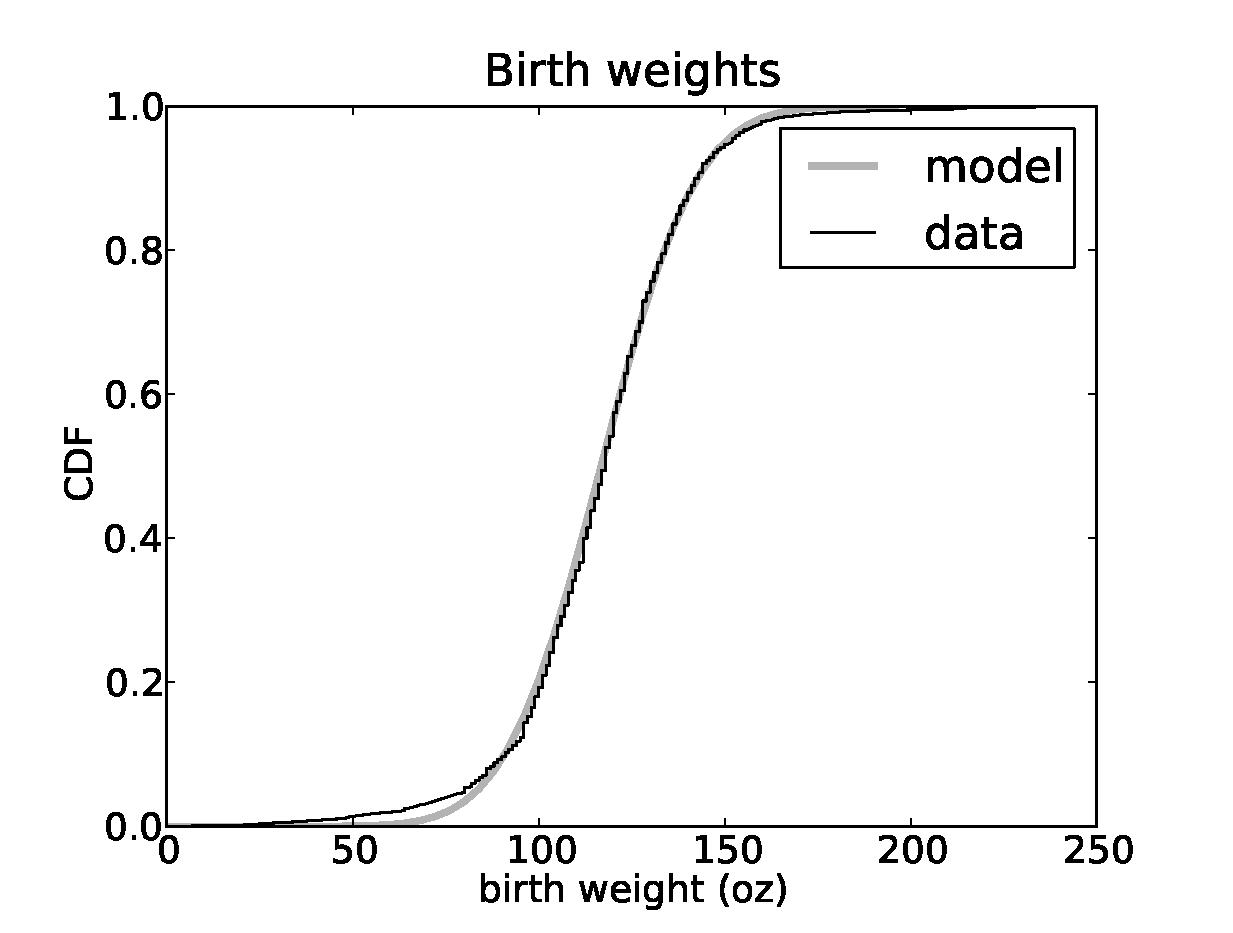
\includegraphics[height=2.5in]{workspace/nsfg_birthwgt_model.eps}}
\caption{CDF of birth weights.}
\label{nsfg_birthwgt_model}
\end{figure}

The normal distribution is a good model for this dataset.  A {\bf
  model} is a useful simplification.  In this case it is useful
because we can summarize the entire distribution with just two
numbers, $\mu=116.5$ and $\sigma=19.9$, and the resulting error
(difference between the model and the data) is small.

Below the 10th percentile there is a discrepancy between the data
and the model; there are more light babies than we would expect in
a normal distribution.  If we are interested in studying preterm
babies, it would be important to get this part of the distribution
right.  In that case it might not be appropriate to use the normal
model.

\begin{ex}
The Wechsler Adult Intelligence Scale is a test that is intended
to measure intelligence\footnote{Whether it does or not is a
fascinating controversy that I invite you to investiage at your
leisure.}.  Results are normalized so that the distribution of scores
in the general population is normal with $\mu=100$ and $\sigma=15$.

Use {\tt erf.NormalCdf} to investigate the frequency of rare events
in a normal distribution.
What fraction of the population has an IQ greater than the mean?
What fraction is over 115?  130?  145?

A ``six-sigma'' event is a value that exceeds the mean by 6 standard
deviations, so a six-sigma IQ is 190.  In a world of 6 billion people,
how many do we expect to have an IQ of 190 or more?
\end{ex}


\begin{ex}
Plot the CDF of pregnancy lengths for all live births.  Does it
look like a normal distribution?

Compute the mean and variance of the sample and plot the normal
distribution with the same parameters.  Is the normal distribution a
good model for this data?  If you had to summarize this distribution
with two statistics, what statistics would you choose?
\end{ex}


\section{Normal probability plot}

For the exponential, Pareto and Weibull distributions, there are
simple transformations we can use to test whether a continuous
distribution is a good model of a dataset.

For the normal distribution there is no such transformation, but there
is an alternative called a {\bf normal probability plot}.  It is based
on {\bf rankits}: if you generate $n$ values from a normal
distribution and sort them, the $k$th rankit is the mean of the
distribution for the $k$th value.

\begin{ex}
This exercise is optional, but it might help you get your head around rankits.

Write a function called {\tt Sample} that generates 6 samples from a
normal distribution with $\mu = 0$ and $\sigma = 1$.  Sort and return
the values.

Write a function called {\tt Samples} that calls {\tt Sample} 1000 times and
returns a list of 1000 lists.

If you apply {\tt zip} to this list of lists, the result is 6 lists
with 1000 values in each.  Compute the mean of each of these lists
and print the results.  I predict that you will get something like
this:

\[ -1.2672,   -0.6418,   -0.2016,   0.2016,   0.6418,   1.2672 \]

If you increase the number of times you call {\tt Sample}, the
results should converge on these values.

\end{ex}

% Algorithms for exact and approximate normal rank stats
% http://download.osgeo.org/grass/grass6_progman/as177_8c_source.html

Computing rankits exactly is moderately difficult, but there are
numerical methods for approximating them.  Also, there is a
quick-and-dirty method that is even easier to implement:

\begin{description}

\item Sort the values in the dataset.

\item From a normal distribution with $\mu = 0$ and $\sigma = 1$,
generate a sample with the same size as your dataset and sort it.

\item Plot the values from your dataset versus the random values.

\end{description}

For large datasets, this method actually does pretty well.
For smaller datasets, you can improve it by generating $m (n+1) - 1$
values from a normal distribution, where $n$ is the size of the
dataset and $m$ is a multiplier.  Then select every $m$th element,
starting with the $m$th.  Hint: use the Python slice operator.

This method works with other distributions as well, as long as
you know how to generate a random sample.

Figure~\ref{nsfg_birthwgt_normal} is a quick-and-dirty normal
probability plot for the birth weight data.

\begin{figure}
% cumulative.py
\centerline{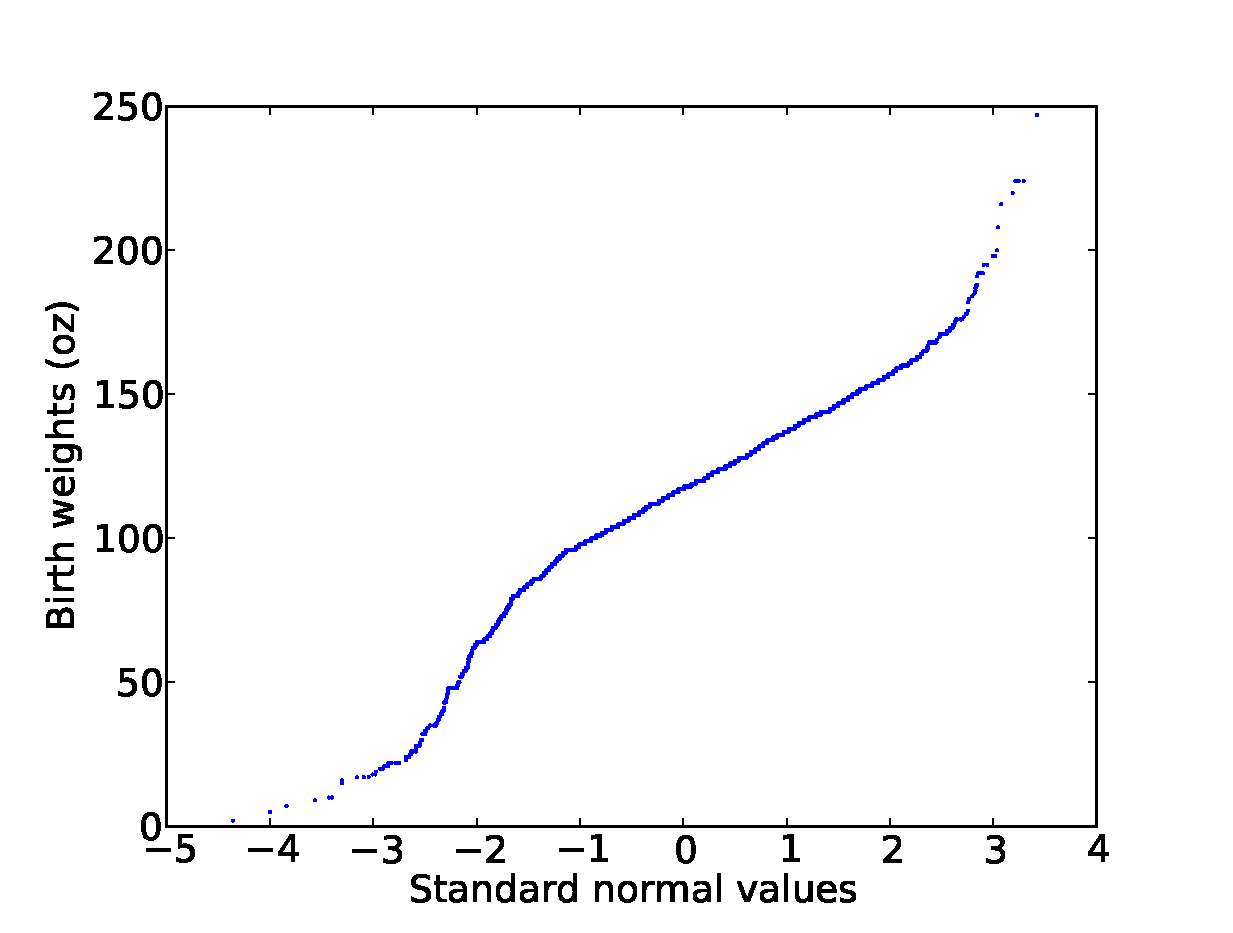
\includegraphics[height=2.5in]{workspace/nsfg_birthwgt_normal.eps}}
\caption{Normal probability plot of birth weights.}
\label{nsfg_birthwgt_normal}
\end{figure}

The curvature in this plot suggests that there are consistent
deviations from a normal distribution; nevertheless, it is a
good (enough) model for many purposes.

\begin{ex}
Sketch a line to fit this curve as well as you can, and
eyeball the slope and intercept.  What meaning do these parameters have?
\end{ex}


\section{The lognormal distribution}
\label{lognormal}

The National Center for Chronic Disease Prevention and Health
Promotion conducts an annual survey as part of the Behavioral Risk
Factor Surveillance System (BRFSS)\footnote{Centers for Disease
  Control and Prevention (CDC). Behavioral Risk Factor Surveillance
  System Survey Data. Atlanta, Georgia: U.S. Department of Health and
  Human Services, Centers for Disease Control and Prevention, 2008.}.
In 2008, they interviewed 414,509 respondents and asked about their
demographics, health and (as the name suggests) health risks.

Among the data they collected are the weights, in kilograms, of
398,484 respondents.  Figure~\ref{brfss_weight_model} shows the
distribution of these weights and a normal model with the same mean
and variance.

\begin{figure}
\centerline{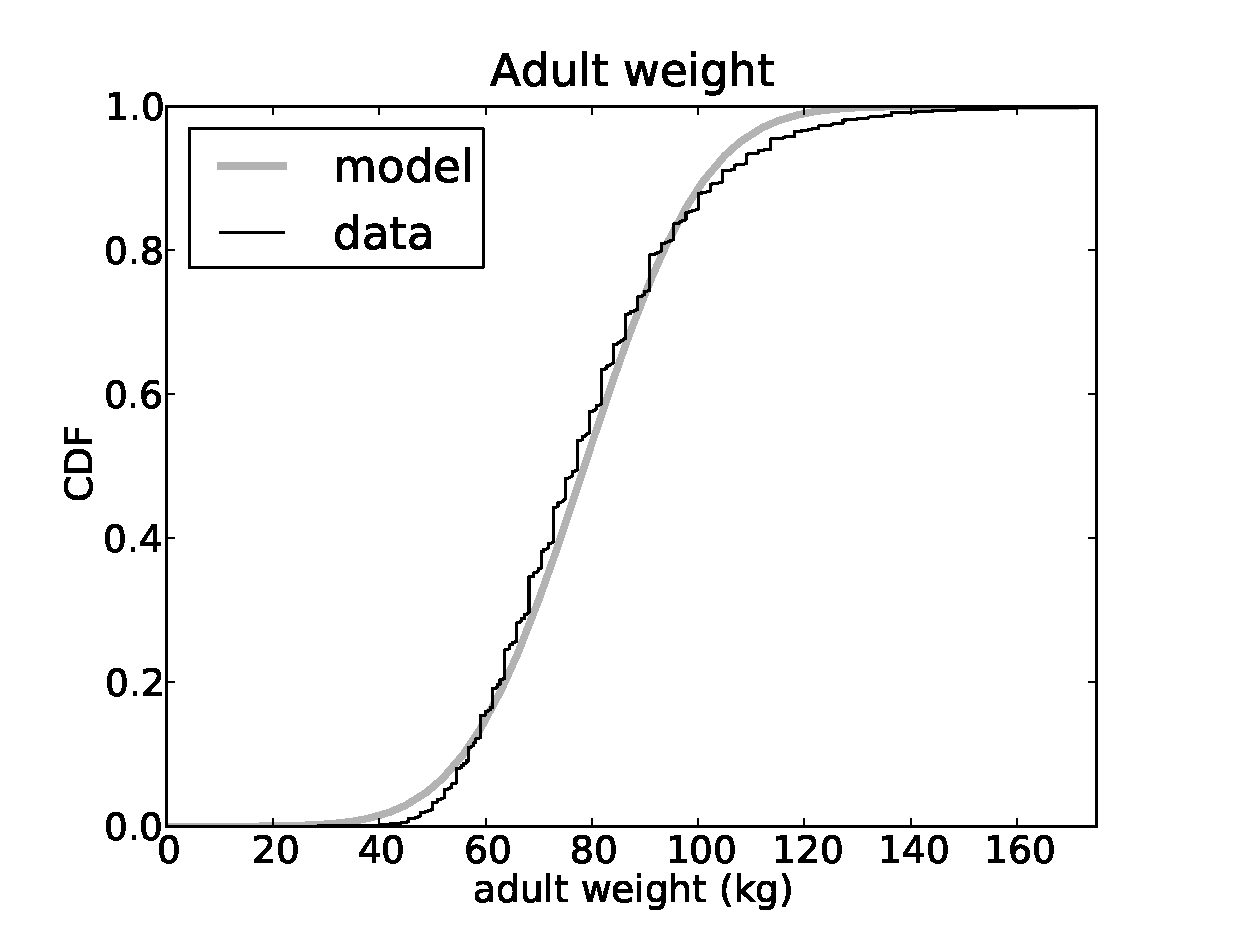
\includegraphics[height=2.5in]{workspace/brfss_weight_model.eps}}
\caption{CDF of adult weights from the BRFSS.}
\label{brfss_weight_model}
\end{figure}

The agreement between the data and the model might be good enough
for some purposes, but there are clear discrepancies below the 10th
and above the 90th percentile.

It turns out that we can do better by applying a logarithmic
transformation\footnote{I was tipped off to this possibility by a
  comment (without citation) at
  \url{mathworld.wolfram.com/LogNormalDistribution.html}.
  Subsequently I found a paper that proposes the log transform and
  suggests a cause: Penman and Johnson, ``The Changing Shape of the
  Body Mass Index Distribution Curve in the Population,'' Preventing
  Chronic Disease, 2006 July; 3(3): A74.  Online
  at\url{www.ncbi.nlm.nih.gov/pmc/articles/PMC1636707}}.
Figure~\ref{brfss_weight_log} shows the distribution
of $\log w$, where $w$ is weight in kilograms, along with a normal
model.

\begin{figure}
\centerline{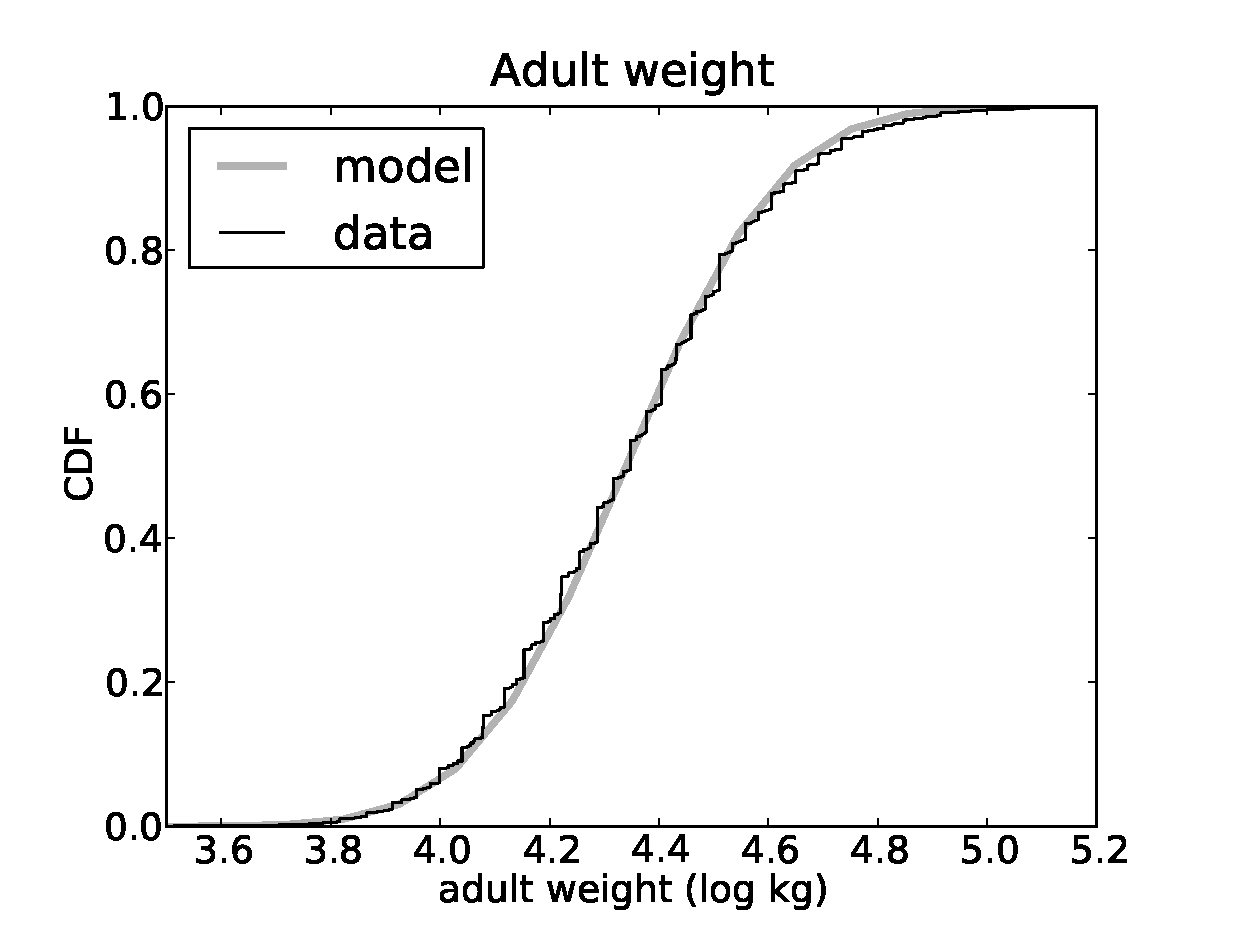
\includegraphics[height=2.5in]{workspace/brfss_weight_log.eps}}
\caption{CDF of adult weights with a log transform.}
\label{brfss_weight_log}
\end{figure}

The normal model is a good fit for the data (although the
highest weights exceed the expectation of the normal model even after
the log transform).

If the log transform fits a normal model, that means that the data
fit a lognormal model.

%In Chapter~\ref{correlation} we will come back
%and look at a possible explanation of this phenomenon.

\begin{ex}

You can download code to work with the BRFSS dataset from \url{}.
General normal probability plots for $w$ and $\log w$.

\end{ex}

\begin{ex}
The distribution of populations for cities and towns has been proposed
as an example of a real-world phenomenon that can be described
with a Pareto distribution.

The U.S.~Census Bureau publishes data on the population of every
incorporated city and town in the United States.  I have written a
small program that downloads this data and stores it in a file.  You
can download it from \url{thinkstatsbook.com/populations.py}.

\begin{enumerate}

\item Read over the program to make sure you know what it does and then
  write a program that computes and plots the distribution of
  populations for the 14,593 cities and towns in the dataset.

\item Plot the CDF on linear and log-$x$ scales so you can get a sense
  of the shape of the distribution.  Then plot the CCDF on a log-log
  scale to see if it has the characteristic shape of a Pareto
  distribution.

\item Try out the other transformations and plots in this chapter to
  see if there is a better model for this data.

\end{enumerate}

What conclusion do you draw about the distribution of sizes
for cities and towns?

\end{ex}


\section{Skewness}

{\bf Skewness} is a statistic that measures the asymmetry of a
distribution.  Given a sequence of values, $x_i$, the sample skewness
is:

\[ g_1 = \frac{m_3}{m_2^{3/2}}\]

\[ m_2 = \frac{1}{n} \sum_i (x_i - \mu)^2 \]

\[ m_3 = \frac{1}{n} \sum_i (x_i - \mu)^3 \]

You might recognize $m_2$ as the mean squared deviation (also known as
variance); similarly, $m_3$ is the mean cubed deviation.

In theory, negative skewness indicates that a distribution 
``skews left;'' that is, it extends
farther to the left than the right.  Positive skewness indicates
that a distribution skews right.

In practice, computing the skewness of a sample is usually not
a good idea.  If there are any outliers, they tend to
have a disproportionate effect on $g_1$.

Another way to evaluate the asymmetry of a distribution is to look
at the relationship between the mean and median.
Extreme values have more effect on the mean than the median, so
in a distribution that skews left, the mean is less than the median.

Pearson's median skewness coefficient is an alternative measure
of skewness:

\[ g_p = 3 (\mu - \mu_{1/2}) / \sigma \]

where $\mu_{1/2}$ is the median of the sample.  This statistic is {\bf
  robust}, which means that it is less vulnerable to the effect of
outliers.

\begin{ex}

In {\tt thinkstats.py} add a function named {\tt Skewness} that computes
$g_1$ for a sample.

Compute the skewness for the distributions of pregnancy length and
birth weight.  Are the results consistent with the shape of the
distributions?

Write a function named {\tt PearsonSkewness} that computes $g_p$
for these distributions.  How does $g_p$ compare to $g_p$?

\end{ex}


\begin{ex}

The ``Lake Wobegon effect'' is an amusing nickname\footnote{If you
  don't get it, see \url{wikipedia.org/wiki/Lake_Wobegon}.} for {\bf
  illusory superiority}, which is the tendency for people to
overestimate their abilities relative to others.  For example, in some
surveys, more than 80\% of respondents believe that they are better
than the average driver\footnote{See
  \url{wikipedia.org/wiki/Illusory_superiority}.}.

If we interpret ``average'' to mean median, then this result is
logically impossible (proof left as an exercise for the reader).
But if ``average'' is the mean, this result is actually possible,
although unlikely. 

The Current Population Survey (CPS) is a joint effort between the
Bureau of Labor Statistics and the Census Bureau.  Data from the
survey are available from \url{www.census.gov/cps/}.

Extract the distribution of incomes from this dataset.  Are any of
the continuous distributions in this chapter a good model of
the data?

Compute the median, mean, skewness and Pearson's skewness.  What
fraction of the population is below the mean?

Optional: The Gini coefficient is often used as a measure of income
inequality.  Read about it at
\url{wikipedia.org/wiki/Gini_coefficient} and write a function called
    {\tt Gini} that computes it for the income distribution.

\end{ex}


\section{Convolution}

What happens when we add these things up?

\section{Central limit theorem}

What happens when we add up a lot of values?

What happens when we multiply out a lot of values?


\section{Glossary}

\begin{description}

\item[empirical distribution:] The distribution of values in a sample.

\item[continuous distribution:] A distribution described by a continuous
function.

\item[interarrival time:] The elapsed time between two events.

\item[error function:] A special mathematical function, so-named
  because it comes up in the study of measurement errors.

\item[normal probability plot:] A plot of the sorted values in a sample
versus the expected value for each if their distribution is normal.

\item[rankit:] The expected value of an element in a sorted list of
values from a normal distribution.

\item[model:] A useful simplification.  Continuous distributions are
often good models of more complex empirical distributions.

\item[skewness:] A characteristic of a distribution; intuitively, it
is a measure of how asymmetric the distribution is.

\item[robust:] A statistic is robust if it is relatively immune to the
effect of outliers.

\item[illusory superiority:] The tendency of people to imagine that
they are better than average.

\item[corpus:] A body of text used as a sample of a language.

\item[hapaxlegomenon:] A word that appear only once in a corpus.
It appears twice in this book, so far.

\end{description}



\chapter{Probability}
\label{probability}

In Chapter~\ref{descriptive}, I said that a probability is a frequency
expressed as a fraction of the sample size.  That's one definition of
probability, but it's not the only one.  In fact, the meaning
of probability is a topic of surprising controversy.

We'll start with the uncontroversial parts and work our way up.  There
is general agreement that a probability is a real value between 0 and
1 that is intended to be a quantitative measure corresponding to the
qualitative notion that some things are more likely than others.

The ``things'' we assign probabilities to are called {\bf events}.  If
$E$ represents an event, then $P(E)$ represents the probability that
$E$ will occur.  A situation where $E$ might or might not happen is
called a {\bf trial}.

As an example, suppose you have a standard six-sided
die\footnote{``Die'' is the singular of ``dice''.} and want to know
the probability of rolling a 6.  Each roll is a trial.
Each time a 6 appears is considered a {\bf success}; other trials are
considered {\bf failures}.  These terms are used even in scenarios
where ``success'' is bad and ``failure'' is good.

If we have a finite sample of $n$ trials and we observe $s$ successes,
the probability of success is $s/n$.  If the set of trials is
infinite, defining probabilities is a little trickier, but most people
are willing to accept probablistic claims about a hypothetical series
of identical trials, like tossing a coin or rolling a die.

We start to run into trouble when we talk about probabilities of
unique events.  For example, we might like to know the probability
that a candidate will win an election.  But every election is unique,
so there is no series of identical trials to consider.

In cases like this some people would say that the notion of
probability does not apply.  This position is sometimes called {\bf
  frequentism} because it defines probability in terms of frequencies.
If there is no set of identical trials, there is no probability.

Frequentism is relatively safe, from a philosophic point of view, but
frustrating because it limits the scope of probability to physical
systems that are either random (like atomic decay) or so unpredictable
that we model them as random (like a tumbling die).  Anything involving
people is pretty much off the table.

An alternative is {\bf Bayesianism}, which defines probability as
a degree of belief that an event will occur.  By this definition,
the notion of probability can be applied in almost any circumstance.
One difficulty with Bayesian probability is that it depends on
a person's state of knowledge; people with different information
might have different degrees of belief about the same event.  For
this reason, many people think that Bayesian probabilities are
(at least more) subjective than frequency probabilities.

As an example, what is the probability that Thaksin Shinawatra is the
Prime Minister of Thailand?  A frequentist would say that there is no
well-defined probability for this event because there is no set of
trials.  Thaksin either is, or is not, the PM; it's not a question of
probability.

In contrast, a Bayesian would be willing to assign a probability to
this event based on his or her state of knowledge.  For example, if
you remember that there was a coup in Thailand in 2006, and you are
pretty sure Thaksin was the PM who was ousted, you might
assign a probability like $0.1$, which acknowledges the possibility
that your recollection is incorrect, or that Thaksin has been
reinstated.

If you consult the Wikipedia, you will learn that Thaksin is not the
PM of Thailand (at least at the time I am writing).  Based on this
information, you might revise your probability estimate to $0.01$,
reflecting the possibility that the Wikipedia is wrong.


\section{Rules of probability}

For frequency probabilities, we can derive rules that relate
probabilities of different events.  Probably the best known of these
rules is

\renewcommand{\and}{\wedge}

\[ P(A \and B) = P(A) P(B) \]

where $P(A \and B)$ is the probability that events $A$ and $B$ both
occur.  This formula is easy to remember, but it only applies if $A$
and $B$ are {\bf independent}, which means that if I know $A$
occurred, that doesn't change the probablility of $B$, and vice versa.

For example, if $A$ is tossing a coin and getting heads, and $B$
is rolling a die and getting 1, $A$ and $B$ are independent, because
the coin toss doesn't tell me anything about the die roll, and vice
versa.

But if I roll two dice, and $A$ is getting at least one six, and
$B$ is getting two sixes, $A$ and $B$ are not independent, because
if I know that $A$ occurred, the probability of $B$ is higher, and
if I know $B$ occurred, the probability of $A$ is 1.

When $A$ and $B$ are not independent, it is often useful to compute
the conditional probability, $P(A|B)$, which is the probability of
$A$ given that we know $B$ occurred

\[ P(A|B) = \frac{P(A \and B)}{P(B)} \]

From that we can derive the general relation

\[ P(A \and B) = P(A) P(B|A) = P(B) P(A|B) \]

This might not be as easy to remember, but if you read it a few times,
it should make sense.  This relationship holds whether $A$ and $B$
are independent or not.

Because all probabilities are in the range from 0 to 1, it is
easy to show that 

\[ P(A \and B) \le P(A) \]

To picture this, imagine a club that only admits people
who satisfy some requirement, $A$.  Now suppose they add a new
requirement for membership, $B$.  It seems obvious that the club
will get smaller, or stay the same if it happens that all the
members satisfy $B$.

But there are some scenarios where people are surprisingly bad at this
kind of analysis.  For examples and discussion of this phenomenon, see
\url{wikipedia.org/wiki/Conjunction_fallacy}.


\begin{ex}

If I roll two dice and the total is 8, what is the chance that
one of the dice is a 6?

\end{ex}

\begin{ex}

The following questions are adapted from Mlodinow, {\em The Drunkard's
  Walk}.

\begin{enumerate}

\item If a family has two children, what is the chance that they
  have two girls?

\item If a family has two children and we know that at least one of
  them is a girl, what is the chance that they have two girls?

\item If a family has two children and we know that the older one is a
  girl, what is the chance that they have two girls?

\item If a family has two children and we know that at least one of
  them is a girl named Florida, what is the chance that they have
  two girls?

\end{enumerate}

You can assume that the probability that any child is a girl is $1/2$,
and that the children in a family are independent trials (in more ways
than one).  You can also assume that the percentage of girls named
Florida is small.

\end{ex}


\section{Monty Hall}

The Monty Hall problem might be the most contentious question in
the history of probability.  The scenario is simple, but the correct
answer is so counterintuitive that many people just can't accept
it, and many smart people have embarrassed themselves not just by
getting it wrong but by arguing the wrong side, aggressively,
in public.

Monty Hall was the original host of the game show {\em Let's Make a
Deal}.  The Monty Hall problem is based on one of the regular
games on the show.  If you are on the show, here's what happens:

\begin{itemize}

\item Monty shows you three closed doors and tells you that there is a
  prize behind each door: one prize is a car, the other two are less
  valuable prizes like peanut butter and fake finger nails.  The
  prizes are arranged at random.

\item The object of the game is to guess which door has the car.  If
  you guess right, you get to keep the car.

\item So you pick a door, which we will call Door A.  We'll call the
  other doors B and C.

\item Before opening the door you chose, Monty likes to increase the
  suspense by opening either Door B or C, whichever does not
  have the car.  (If the car is actually behind Door A, Monty can
  safely open B or C, so he chooses one at random).

\item Then Monty offers you the option to stick with your original
  choice or switch to the one remaining unopened door.

\end{itemize}

The question is, should you ``stick'' or ``switch'' or does it
make no difference?

Most people have the very strong intuition that it makes no difference.
There are two doors left, they reason, so the chance that the car
is behind Door A is 50\%.

But that is wrong.  In fact, the chance of winning if you stick
with Door A is only 1/3; if you switch, your chances are 2/3.
I will explain why, but I don't expect you to believe me.

The key is to realize that there are three possible scenarios:
the car is either behind Door A, B or C.  Since the prizes are
arranged at random, the probability of each scenario is 1/3.

If your strategy is to stick with Door A, then you will only
win in Scenario A, which has probability 1/3.

If your strategy is to switch, you will win in either Scenario
B or Scenario C, so the total probability of winning is 2/3.

\newcommand{\Erdos}{Erd\H{o}s}

If you are not completely convinced by this argument, you are
in good company.  When a friend presented this solution to
Paul \Erdos, he replied, ``No, that is impossible.  It should
make no difference.\footnote{See Hoffman, {\em The Man Who Loved
Only Numbers}, page 83.}''

No amount of argument could convince him.  In the end, it took
a computer simulation to bring him around.

\begin{ex}

Write a program that simulates the Monty Hall problem and use
it to estimate the probability of winning if you stick, and if
you switch.

Then read the discussion of the problem at
\url{wikipedia.org/wiki/Monty_Hall_problem}.

Which do you find more convincing, the simulation or the arguments,
and why?

\end{ex}


\begin{ex}

To understand the Monty Hall problem, it is important to realize
that by deciding which door to open, Monty is giving you information.
To see why this matters, imagine the case where Monty doesn't
know where the prizes are, so he chooses Door B or C at random.

If he opens the door with the car, the game is over, you lose, and
you don't get to choose whether to switch or stick.

Otherwise, are you better off switching or sticking?

\end{ex}



\newcommand{\Poincare}{Poincar\'{e}}

\section{\Poincare}

Henri \Poincare~was a French mathematician who taught at the Sorbonne
from 1881 until his death in 1912.  The following anecdote about him
is probably apocryphal, but it makes an interesting probability
problem.

Supposedly \Poincare~suspected that his local bakery was selling
loaves of bread that were lighter than the advertised weight of 1 kg,
so every day for a year he bought a loaf of bread, brought it home and
weighed it.  At the end of the year, he plotted the distribution of
his measurements and showed that it fit a normal distribution with
mean 950 g and standard deviation 50 g.  He brought this evidence to
the bread police, who gave the baker a warning.

For the next year, \Poincare~continued the practice of weighing his
bread every day.  At the end of the year, he found that the average
weight was 1000 g, just as it should be, but again he complained to
the bread police, and this time they fined the baker.

Why?  Because the shape of the distribution was asymmetric.  Unlike
the normal distribution, it was skewed to the right, which is
consistent with the hypothesis that the baker was still making 950 g
loaves, but deliberately giving \Poincare~the heavier ones.


\begin{ex}

Write a program that simulates a baker who chooses $n$ loaves from a
distribution with mean 950 g and standard deviation 50 g, and gives
the heaviest one to \Poincare.  What value of $n$ yields a
distribution with mean 1000 g?  What is the standard deviation?

Compare this distribution to a normal distribution with the same mean
and the same standard deviation.  Is the difference in the shape of
the distribution big enough to convince the bread police?

\end{ex}


\begin{ex}

If you go to a dance where partners are paired up randomly, what
percentage of opposite sex couples will you see where the woman is
taller than the man?

In the BRFSS (see Section~\ref{lognormal}), the distribution of
heights is roughly normal with parameters $\mu=178$ cm and
$\sigma=59.4$ cm for men, and $\mu=163$ cm and $\sigma=52.8$ cm for
women.

As an aside, you might notice that the standard deviation for men is
higher and wonder whether men's heights are more variable.  To compare
variability between groups, it is useful to compute the {\bf
  coefficient of variation}, which is the standard deviation as a
fraction of the mean, $\mu / \sigma$.  By this measure, women's
heights are slightly more variable.

% From brfss.py
%    mean          var           std           cv
% 1 178.090966766 59.4275328443 7.70892553112 0.0432864488925
% 2 163.226104443 52.7684723388 7.26419110011 0.0445038563217

\end{ex}


\section{Streaks and hot spots}

People do not have very good intuition for random processes.  If you
ask people to generate ``random'' numbers, they tend to generate
sequences that are random-looking, but actually more ordered than real
random sequences.  Conversely, if you show them a real random
sequence, they tend to see patterns where there are none.

An example of the second phenomenon is the prevalence of belief
in ``streaks'' in sports: a player that has been successful recently
is said to have a ``hot hand;'' a player that has been unsuccessful is
``in a slump.''

Statisticians have tested these hypotheses in a number of sports, and
the consistent result is that there is no such thing as a
streak\footnote{For example, see Gilovich, Vallone and Tversky, ``The
  hot hand in basketball: On the misperception of random sequences,''
  1985.}.  If you assume that each attempt is independent of previous
attempts, you will see occasional long strings of successes or
failures.  These apparent streaks are not sufficient evidence that
there is any correlation between successive attempts.

A related phenomenon is the clustering illusion, which is the
tendency to see clusters in spatial patterns that are actually
random (see \url{wikipedia.org/wiki/Clustering_illusion}).
Monte Carlo simulations are a useful way to test whether an apparent
cluster is likely to be meaningful.

\begin{ex}

If there are 10 players in a basketball game and each one takes
15 shots during the course of the game, and each shot has a
50\% probability of going in, what is the probability that 
you will see, in a given game, at least one player who
hits 10 shots in a row?  If you watch a season of 82 games,
what are the chances you will see at least one streak of
10 hits or misses?

This problem demonstrates some strengths and weaknesses of Monte
Carlo simulation.  A strength is that it is often easy and fast
to write a simulation, and no great knowledge of probability is
required.  A weakness is that estimating the probability of
rare events can take a long time!  A little bit of analysis can
save a lot of computing.

\end{ex}


\begin{ex}

In 1941 Joe DiMaggio got at least one hit
in 56 consecutive games\footnote{See
  \url{wikipedia.org/wiki/Hitting_streak}.}.  Many baseball fans
consider this streak the greatest achievement in any sport in history,
because it was so unlikely.

Use a Monte Carlo simulation to estimate the probability that
any player in major league baseball will have a hitting streak
of 57 or more games in the next century.

\end{ex}


\begin{ex}

A cancer cluster is defined by the Centers for Disease Control (CDC)
as ``greater-than-expected number of cancer cases that occurs within a
group of people in a geographic area over a period of
time.\footnote{From \url{cdc.gov/nceh/clusters/about.htm}.}''

Many people interpret a cancer cluster as evidence of an environmental
hazard, but many scientists and statisticians think that investigating
cancer clusters is a waste of time\footnote{See Gawande, ``The Cancer
  Cluster Myth,'' {\em New Yorker}, Feb 8, 1997.}.  Why?  One reason
(among several) is that identifying cancer clusters is a classic case
of the Sharpshooter Fallacy (see
\url{wikipedia.org/wiki/Texas_sharpshooter_fallacy}).

Nevertheless, when someone reports a cancer cluster, the CDC is
obligated to investigate.  According to their web page:

\begin{quote}

``Investigators develop a `case' definition, a time period of concern,
  and the population at risk. They then calculate the expected number
  of cases and compare them to the observed number. A cluster is
  confirmed when the observed/expected ratio is greater than 1.0, and
  the difference is statistically significant.''

\end{quote}

\begin{enumerate}

\item Suppose that a particular cancer has an incidence of 1 case per
  thousand people per year.  If you follow a particular cohort of 100
  people for 10 years, you would expect to see about 1 case.  If you
  saw two cases, that would not be very surprising, but more than than
  two would be rare.

Write a program that simulates a large number of cohorts over
a 10 year period and estimates the distribution of total cases.

\item An observation is considered statistically significant if its
  probability by chance alone, called a $p$-value, is less than 5\%.
  In a cohort of 100 people over 10 years, how many cases would you
  have to see to meet this criterion?

\item Now imagine that you divide a population of 10000 people into 100
  cohorts and follow them for 10 years.  What is the chance that at
  least one of the cohorts will have a ``statistically significant''
  cluster?  What if we require a $p$-value of 1\%.?

\item Now imagine that you arrange 10000 people in a 100 $\times$ 100
  grid and follow them for 10 years.  What is the chance that there
  will be at least one 10 $\times$ 10 block anywhere in the grid
  with a statistically significant cluster?

\item Finally, imagine that you follow a grid of 10000 people for 30
  years.  What is the chance that there will be a 10-year interval
  at some point with a 10 $\times$ 10 block anywhere in the grid
  with a statistically significant cluster?

\end{enumerate}

\end{ex}



\section{Bayes' theorem}

Bayes' theorem is a relationship between the conditional probabilities
of two events.  A conditional probability, often written $P(A|B)$ is
the probability that Event A will occur given that we know that
Event B has occurred.  Bayes' theorem states:

\[ P(A|B) = \frac{P(B|A)P(A)}{P(B)} \]

To see that this is true, it helps to write $P(A \and B)$, which
is the probability that A and B occur

\[ P(A \and B) = P(A) P(B|A) \]

But it is also true that 
 
\[ P(A \and B) = P(B) P(A|B) \]

So

\[ P(B) P(A|B) = P(A) P(B|A) \]

Dividing through by $P(B)$ yields Bayes' theorem.

Bayes' theorem is often interpreted as a statement about 
how a body of evidence, $E$, affects the probability of a 
hypothesis, $H$:

\[ P(H|E) = P(H) \frac{P(E|H)}{P(E)} \]

In words, this equation says that the probability of $H$ after you
have seen $E$ is the product of $P(H)$, which is the probability of
$H$ before you saw the evidence, and the ratio of $P(E|H)$, the
probability of seeing the evidence assuming that $H$ is true, and
$P(E)$, the probability of seeing the evidence under any circumstances
($H$ true or not).

This way of reading Bayes' theorem is called the ``diachronic''
interpretation because it describes how the probability of a
hypothesis gets updated, over time, in light of new evidence.  In this
context, $P(H)$ is called the {\bf prior} probability and $P(H|E)$ is
called the {\bf posterior}.  The update term $P(E|H)/P(E)$ is called
the {\bf likelihood ratio}.

A classic use of Bayes' Theorem is the interpretation of clinical
tests.  For example, routine testing for illegal drug use is
increasingly common in workplaces and schools (See
\url{aclu.org/drugpolicy/testing/index.html}.).  The companies that
perform these tests maintain that the tests are sensitive, which means
that they are likely to produce a positive result if there are drugs
(or metabolites) in a sample, and specific, which means that they are
likely to yield a negative result if there are no drugs.

Studies from the Journal of the American Medical
Association\footnote{I got these number from Gleason and Barnum,
  ``Predictive Probabilities In Employee Drug-Testing,'' at
  \url{piercelaw.edu/risk/vol2/winter/gleason.htm}.} estimate that
the sensitivity of common drug tests is about 60\% and the specificity
is about 99\%.

Now suppose these tests are applied to a workforce where the
actual rate of drug use is 5\%.  Of the employees who test positive,
how many of them actually use drugs?

In Bayesian terms, we want to compute the probability of
drug use given a positive test, $P(D|+)$.  By Bayes' Theorem:

\[ P(D|+) = P(D) \frac{P(+|D)}{P(+)} \]

The prior, $P(D)$ is the probability of drug use before we
see the outcome of the test, which is 5\%.
The numerator of the likelihood ratio, $P(+|D)$, is the probability
of a positive test assuming drug use, which is the sensitivity.

The denominator, $P(+)$ is a little harder to evaluate.  We have to
consider two possibilities, $P(+|D)$ and $P(+|N)$, where $N$ is the
hypothesis that the subject of the test does not use drugs:

\[ P(+) = P(D) P(+|D) + P(N) P(+|N) \]

The probability of a false positive, $P(+|N)$, is the complement
of the specificity, or 1\%.

Putting it together, we have

\[ P(D|+) = \frac{P(D) P(+|D)}{P(D) P(+|D) + P(N) P(+|N)}\]

Plugging in the given values yields $P(D|+) = 0.76$, which means
that of the people who test positive, about 1 in 4 is innocent. 

\begin{ex}

Write a program that takes the actual rate of drug use, and the
sensitivity and specificity of the test, and uses Bayes' Theorem
to compute $P(D|+)$.

Suppose the same test is applied to a population where the actual
rate of drug use is 1\%.  What is the probability that someone
who tests positive is actually a drug user?

\end{ex}


\begin{ex}

This exercise is from \url{wikipedia.org/wiki/Bayesian_inference}.

\begin{quote}

``Suppose there are two full bowls of cookies. Bowl 1 has 10 chocolate
  chip and 30 plain cookies, while Bowl 2 has 20 of each. Our friend
  Fred picks a bowl at random, and then picks a cookie at random. The
  cookie turns out to be a plain one. How probable is it that Fred
  picked it out of Bowl 1?''

\end{quote}

\end{ex}

\begin{ex}

Elvis's twin

Other Examples from MacKay's Chapter 3?

\end{ex}


\section{Glossary}

\begin{description}

\item[:] 

\item[:] 

\item[:] 

\item[:] 

\item[:] 

\item[:] 

\item[:] 

\item[:] 

\end{description}


\chapter{Hypothesis testing}

Exploring the data from the NSFG, we saw several ``apparent effects;''
including a number of differences between first babies and others.
So far we have taken these effects at face value; in this chapter,
finally, we will put them to the test.

The fundamental question we want to address is whether these effects
are real.  For example, if we see a difference in the mean pregnancy
length for first babies and others, we want to know whether that
difference is real, or whether it occurred by chance.

That question turns out to be hard to address directly, so we will
proceed in two steps.  First we will test whether the effect is {\bf
  significant}, then we will try to interpret the result
  as an answer to the original question.

In the context of statistics, ``significant'' has a technical
definition that is different from its use in common language.
As we defined earlier, an apparent effect is statistically
significant if it is unlikely to have occurred by chance.

To make this more precise, we have to answer three questions:

\begin{enumerate}

\item What do we mean by ``chance?''

\item What do we mean by ``unlikely?''

\item What do we mean by ``effect?''

\end{enumerate}

All three of these questions are harder than they look.  Nevertheless,
there is a general structure that people use to test statistical
significance:

\begin{description}

\item[Null hypothesis:] The null hypothesis is a model of the system
  based on the assumption that the apparent effect was actually due to
  chance.

\item[p-value:] The {\bf p-value} is the probability of the apparent
  effect under the null hypothesis.

\item[Interpretation:] Based on the p-value, we conclude that the
  effect is either statistically significant, or not.

\end{description}

This process is called {\bf hypothesis testing}.  The underlying
logic is similar to a proof by contradiction.  To prove a mathematical
statement, A, you can assume, temporarily, that A is false.  If this
assumption leads to a contradiction, you conclude that A must actually
be true.

Similarly, to test a hypothesis like, ``This effect is real,'' we
assume, temporarily, that is is not.  That's the null hypothesis.
Based on that assumption, we compute the probability of the apparent
effect.  That's the p-value.  If the p-value is low enough, we
conclude that the null hypothesis is unlikely to be true.


\section{Testing a difference in means}

One of the easiest hypotheses to test is an apparent difference in mean
between two groups.  In the NSFG data, we saw that the mean pregnancy
length for first babies is slightly longer, and the mean weight at
birth is slightly smaller.  Now we will see if those effects are
significant.

For these examples, the null hypothesis is that the distributions
for the two groups are the same, and that the apparent difference is
due to chance.

To compute p-values, we find the pooled distribution for all live
births (first babies and others), generate random samples that are
the same size as the observed samples, and compute the difference
in means under the null hypothesis.

If we generate a large number of samples, we can count how often the
difference in means (due to chance) is as big or bigger than the
difference we actually observed.  This fraction is the p-value.

For pregnancy length, we observed $n=4413$ first babies and $m=4735$
others, and the difference in mean was $\delta=0.073$.  To estimate
the p-value of this effect, I pooled the distributions, generated
samples with sizes $n$ and $m$ and computed the difference in mean.

This process is called {\bf resampling} because we are drawing a
random sample from a dataset that is, itself, a sample of the general
population.  I computed differences for 1000 sample pairs;
Figure~\ref{length_deltas_cdf} shows their distribution.

\begin{figure}
\centerline{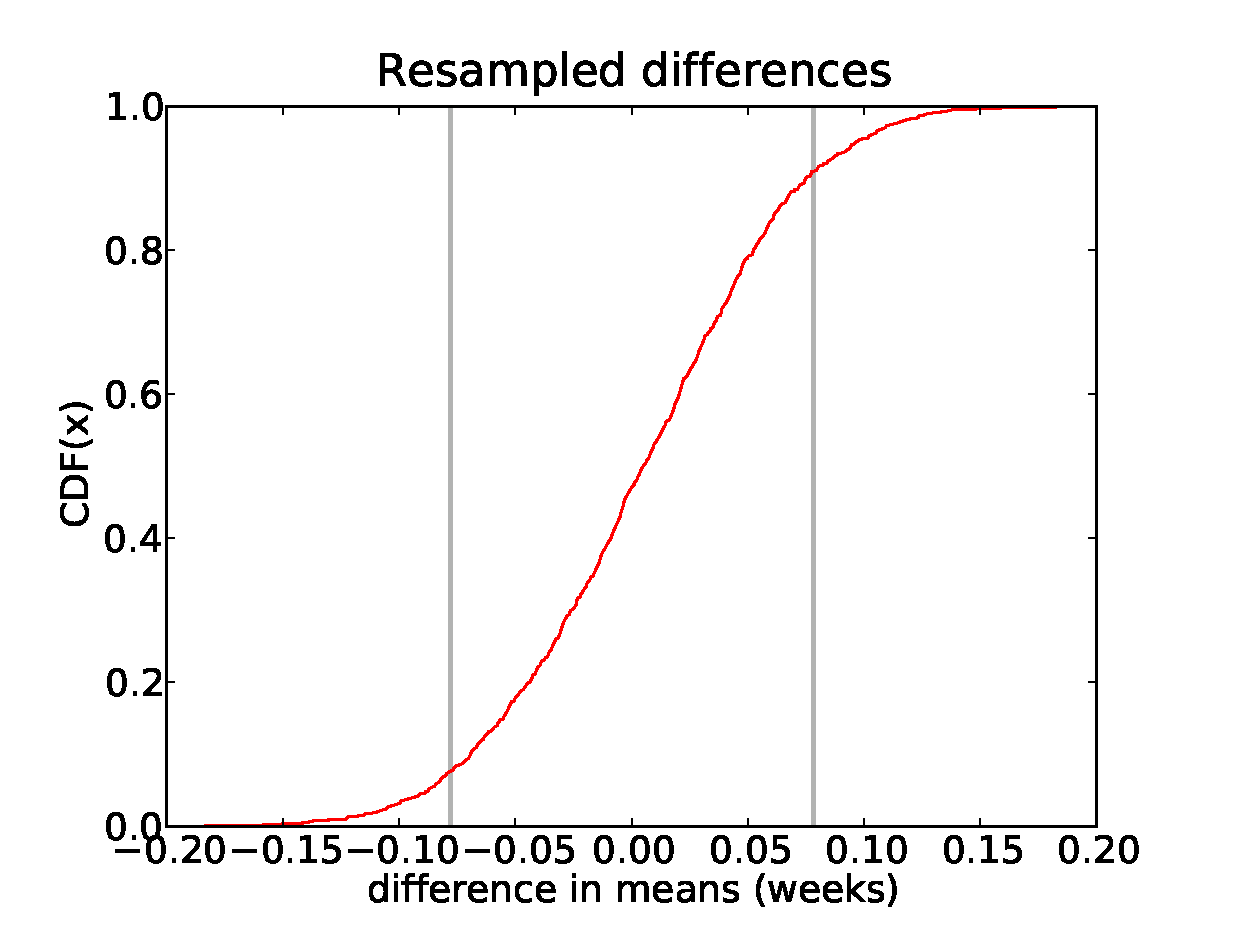
\includegraphics[height=2.5in]{workspace/length_deltas_cdf.eps}}
\caption{CDF of difference in mean for resampled data.}
\label{length_deltas_cdf}
\end{figure}

The mean difference is near 0, as you would expect with samples
from the same distribution.  The vertical lines show the cutoffs where
$x=-\delta$ or $x=\delta$.

Of 1000 sample pairs, there were 127 where the difference in mean
(positive or negative) was as big or bigger than $\delta$, so the
p-value is approximately 0.127.  In other words, we expect to see an
effect as big as $\delta$ 12.7\% of the time, even if the actual
distribution for the two groups is the same.

So the apparent effect is not very likely, but is it unlikely enough?
I'll address that in the next section.

\begin{ex}

In the NSFG dataset, the difference in mean weight for first
births is 2.0 ounces.  Estimate the p-value of this difference.

Hint: for this kind of resampling it is important to sample
with replacement, so you should use {\tt random.choice} rather
than {\tt random.sample}.


%%%%%% Need to go back and introduce sampling with and without replacement.

\end{ex}


\section{Choosing a threshold}
\label{threshold}

In hypothesis testing we have to worry about two kinds of errors.

\begin{itemize}

\item A Type I error, also called a {\bf false positive} is when we
  accept a hypothesis that is actually false; that is, we consider an
  effect significant when it was actually due to chance.

\item A Type II error, also called a {\bf false negative} is when we
  reject a hypothesis that is actually true; that is, we attribute an
  effect to chance when it was actually real.

\end{itemize}

The most common approach to hypothesis testing is to choose a
threshold, $\alpha$, for the p-value and to accept as significant any
effect with a p-value less than $\alpha$.  A common choice for
$\alpha$ is 5\%.  By this criterion, the apparent difference in
pregnancy length for first babies is not significant, but the
difference in weight is.

For this kind of hypothesis testing, we can compute the probability of
a false positive explicitly: it turns out to be $\alpha$.

To see why, think about the definition of false positive---the chance
of accepting a hypothesis that is false---and the definition of a
p-value---the chance of generating the measured effect if the
hypothesis is false.

Putting these together, we can ask: if the hypothesis is false,
what is the chance of generating a measured effect that will be
considered significant with threshold $\alpha$.  The answer is
$\alpha$.

We can decrease the chance of a false positive by decreasing the
threshold.  For example, if the threshold is 1\%, there is only a 1\%
chance of a false positive.

But there is a price to pay: decreasing the threshold raises the
standard of evidence, which increases the chance of rejecting
a valid hypothesis.

In general there is a tradeoff between Type I and Type II errors.
The only way to decrease both at the same time is to increase the
sample size (or, in some cases, decrease measurement error).

\begin{ex}

To investigate the effect of sample size on p-value, see what happens
if you discard half of the data from the NSFG.  Hint: use {\tt
  random.sample}.  What if you discard three-quarters of the data, and
so on?

What is the smallest sample size where the difference in mean birth
weight is still significant with $\alpha=5$\%?  How much
larger does the sample size have to be with $\alpha=1$\%?

\end{ex}


\section{Defining the effect}

When something unusual happens, people often say something like,
``Wow!  What were the chances of {\em that}!''  This question makes
sense because we have an intuitive sense that some things are more
likely than others.  But this intuition doesn't always hold up to
scrutiny.

For example, supposed I toss a coin 10 times, and after each toss I
write down H for heads and T for tails.  If the result was a sequence
like THHTHTTTHH, you would't be to surprised.  But if the result was
HHHHHHHHHH, you would say something like, ``Wow!  What were the
chances of {\em that}!''

For this example, at least, we can answer the question.  The
probability of getting the sequence HHHHHHHHHH is one in 1024.  But
here's the catch: the probability of getting THHTHTTTHH is also one in
1024, and likewise for any other sequence.

So when we ask, ``What were the chances of {\em that},'' we have
to be careful about what we mean by ``that.''

For the NSFG data, I defined the effect as ``a difference in mean
(positive or negative) as big or bigger than $\delta$.''  By making
this choice, I decided to evaluate the magnitude of the difference,
ignoring the sign.

A test like that is called {\bf two-sided}, because we consider both
sides (positive and negative) in the distribution from
Figure~\ref{length_deltas_cdf}.  By using a two-sided test we are
testing the hypothesis that there is a signficant difference between
the distributions, without specifying the sign of the difference.

The alternative is to use a {\bf one-sided} test, which asks whether
the mean for first babies is significanly {\em higher} than
the mean for others.  Because the hypothesis is more specific, the
p-value is lower---in this case it is roughly half.

%%% Do I mean higher or lower?

\section{Interpreting the result}

At the beginning of this chapter I said that the question we want to
address is whether an apparent effect is real.  We started by defining
the null hypothesis, denoted $H_0$, which is the
hypothesis that the effect is not real.  Then we defined the p-value,
which is $P(E | H_0)$, where $E$ is an effect as big as or bigger than
the apparent effect.  Then we computed p-values and compared
them to a threshold, $\alpha$.

That's a useful step, but it doesn't answer the original question,
which is whether the effect is real.  There are several ways to
interpret the result of a hypothesis test:

\begin{description}

\item[Classical:] In classical hypothesis testing, if a p-value
  is less than $\alpha$, you can say that the effect is statistically
  significant, but you can't conclude that it's real.  This
  formulation is careful to avoid leaping to conclusions, but it is
  also deeply unsatisfying.

\item[Practical:] In practice, people are not so formal.  In most
  science journals, researchers report p-values without apology, and
  readers interpret them as evidence that the apparent effect is real.
  The lower the p-value, the higher their confidence in this
  conclusion.

\item[Bayesian:] What we really want to know is $P(H_A | E)$, where
  $H_A$ is the hypothesis that the effect is real.  By Bayes' Theorem

  \[ P(H_A | E) = \frac{P(E | H_A)}{P(E)} P(H_A) \]

  Where $P(H_A)$ is the prior probability of $H_A$ before we saw the
  effect, $P(E | H_A)$ is the probability of seeing $E$, assuming that
  the effect is real, and $P(E)$ is the probability of seeing $E$
  under any hypothesis.  Since the effect is either real or it's not,

  \[ P(E) = P(E | H_A)P(H_A) + P(E | H_0)P(H_0) \]

\end{description}

As an example, I'll compute $P(H_A | E)$ for pregnancy lengths in the
NSFG.  We have already computed $P(E | H_0)=0.127$, so all we have to
do is compute $P(E | H_A)$ and choose a value for the prior.

To compute $P(E | H_A)$, we assume that the effect is real---that is,
that the distributions are different for first babies and others---and
compute the probability of seeing an effect as big or bigger than
$\delta = 0.73$.  By generating 1000 sample pairs, one from each
distribution, I estimated $P(E | H_A) = 0.503$.  With the prior
$P(H_A)=0.5$, the posterior probability of $H_A$ is 0.798.

% P(H_A) = 0.5 * (0.503) / (0.5*0.503 + 0.5*0.127) = 0.79841269841269846

So if the prior probability of $H_A$ is 50\%, the updated
probability, taking into account the evidence from this dataset,
is almost 80\%.  It makes sense that the posterior probability
is higher, since the data provide some support for the hypothesis.
But it might seem surprising that the difference is so large,
especially since we found that the difference in means was not
statistically significant.

In fact, the method we used in this section is not quite right, and
it tends to overstate the impact of the evidence.  In the next section
we will correct this tendency.

\begin{ex}

What is the posterior probability that the distribution of birth
weights is different for first babies and others?

\end{ex}


\section{Cross-validation}

In the previous example, we used the dataset to formulate the
hypothesis $H_A$, and then we used the same dataset to test it.
Methods like this can sometimes be acceptable, but in general
they are risky.

The problem is that even when the null hypothesis is true, there is
likely to be some difference, $\delta$, between any two groups, just
by chance.  If we use the observed value of $\delta$ to formulate
the hypothesis, $P(H_A | E)$ is likely to be high even when $H_A$ is
false.

We can address this problem with {\bf cross-validation}, which uses
one dataset to estimate $\delta$ and a {\em different} dataset to
evaluate $H_A$.  This first dataset is called the {\bf training set};
the second is called the {\bf testing set}.

In a study like the NSFG, which studies a different cohort in each
cycle, we can use one cycle for training and another for testing.
Or we can partition the data into subsets (at random), then use
one for training and one for testing.

I implemented the second approach, dividing the Cycle 6 data roughly
in half.  I ran the test several times with different random partitions.
The average posterior probability was $P(H_A | E) = 0.621$.  As
expected, the impact of the evidence is smaller, partly because of
the smaller sample size in the test set, and also because we are
no longer using the same data for training and testing.

% t = [0.656, 0.622, 0.511, 0.651, 0.665]
% sum(t)/len(t)


\section{Reporting Bayesian probabilities}

In the previous section we chose the prior probability $P(H_A) = 0.5$.
If we have a set of hypothesis and no reason to think one is more
likely than another, it is common to assign each the same probability.

Some people object to Bayesian probabilities because they depend on
prior probabilities, and people might not be able to agree on
the right prior.  For people who expect scientific results to be
objective and universal, this property is deeply unsettling.

One response to this objection is that, in practice, strong evidence
tends to swamp the effect of the prior, so people who start with
different priors will converge toward the same posterior
probability.

Another option is to report just the likelihood ratio, 
$P(H_A | E)/P(E)$, rather than the posterior probability.  That way
readers can plug in whatever prior they like and compute their own
posteriors (no pun intended).


\section{Pregnancy lengths one more time}

In Section~\ref{threshold} we concluded that the apparent difference
in mean pregnancy length for first babies and others was not
significant.  But in Section~\ref{relative.risk}, when we computed
relative risk, we saw that first babies are more likely to be early,
less likely to be on time, and more likely to be late.

So maybe the distributions have the same mean and different variance.
We could test the significance of the difference in variance, but
the variance is less robust than the mean, and hypothesis tests for
variance often behave badly.

An alternative is to test a hypothesis that more directly reflects the
effect as it appears; that is, the hypothesis that first babies are
more likely to be early, less likely to be in time, and more likely to
be late.

We proceed in five easy steps:

\begin{enumerate}

\item We define a set of categories, called {\bf cells}, that each
  baby might fall into.  In this example, there are six cells because
  there are two groups (first babies and others) and three bins
  (early, on time or late).

I'll use the definitions from Section~\ref{relative.risk}: a baby is
early if it is born during Week 37 or earlier, on time if it is born
during Week 38, 39 or 40, and late if it is born during Week 41 or
later.

\item We compute the number of babies we expect in each cell.  Under
  the null hypothesis, we assume that the distributions are the same
  for the two groups, so we can compute the pooled probabilities:
  $p_{early}$, $p_{ontime}$ and $p_{late}$.

For first babies, we have $n=4413$ samples, so under the null hypothesis
we expect $n p_{early}$ first babies to be early, $n p_{ontime}$ to be
on time, etc.  Likewise, we have $m=4735$ other babies, so we expect
$m p_{early}$ other babies to be early, etc.

\item For each cell we compute the deviation; that is, the difference
  between the observed value, $O_i$, and the expected value, $E_i$

\item We compute some measure of the total deviation; the most common
choice is the chi-squared statistic:

  \[ \chi^2 = \sum_i \frac{(O_i - E_i)^2}{E_i} \]

%% Consider using upper case chi, which is more strictly correct,
%% but harder to distinguish from X.

\item We can use a Monte Carlo simulation to compute the p-value,
  which is the probability of seeing a chi-squared statistic as high
  as the observed value under the null hypothesis.

\end{enumerate}

\begin{ex}

Use the data from the ??? to compute $p_{early}$, $p_{ontime}$ and
$p_{late}$.  The compute the $E_i$, $O_i$ and $\chi^2$.  What is the
p-value of $\chi^2$ under the null hypothesis.  According to this
test, is the observed effect statistically significant?

\end{ex}



\section{Efficient resampling}

Using the central limit theorem to compute the distribution of a sample mean.



\section{Power}

Definition

Compute it

Comment on the loss of power in cross-validation due to smaller sample size 

Examples:

   T-test?

   pregnancy length: early vs. on time vs. late

   Chi-squared test

   Test difference in variance?

Pitfalls:

1) Exploring and then testing

2) Multiple tests

3) Publication bias


Solutions:

1) two phases: exploratory and testing, on different data (possibly a subset)

2) Holm-Bonferroni method

3) publish everything and wait for consensus




\section{Glossary}

\begin{description}

\item[:] 

\item[:] 

\item[:] 

\item[:] 

\item[:] 

\item[:] 

\item[:] 

\item[:] 

\end{description}


\chapter{Estimators}

An estimator is a statistic that converges on a parameter.

A statistic is a function that takes a dataset and returns a number.

Confidence intervals, oh my.


\section{Bayesian estimation}



\section{Glossary}

\begin{description}

\item[:] 

\item[:] 

\item[:] 

\item[:] 

\item[:] 

\item[:] 

\item[:] 

\item[:] 

\end{description}


\chapter{Correlation}

In Chapter~\ref{continuous} we saw that the distribution of weight for adults
in the BRFSS is approximately lognormal, and 

rank correlation

Spearman's correlation

least squares fit

Examples:

    weight gain vs. current weight, explanation of lognormal distribution

Goodness of fit for evaluating distribution models

Show CLT rate of convergence to normal for different distributions 
(test linearity on a normal prob graph)


\chapter{Reminders}

moments

modes

   multimodal distributions (artifact examples: heights, gestation)

Gelman's paradox
\url{http://www.iq.harvard.edu/blog/sss/archives/2008/04/gelmans_paradox.shtml}

\printindex

\clearemptydoublepage
%\blankpage
%\blankpage
%\blankpage


\end{document}
